% !TeX encoding = UTF-8
% !TeX TXS-program:compile = txs:///latexmk/{-pdf} -xelatex
% !TeX TXS-program:recompile-bibliography = txs:///latexmk/{} -v

% 载入 SJTUThesis 模版
\documentclass[type=doctor]{sjtuthesis}
% 选项
%   type=[doctor|master|bachelor],     % 可选(默认:master),论文类型
%   zihao=[-4|5],                      % 可选(默认:-4),正文字号大小
%   lang=[zh|en|de|ja],                % 可选(默认:zh),论文的主要语言
%   review,                            % 可选(默认:关闭),盲审模式
%   [twoside|oneside],                 % 可选(默认:twoside),双页或单页边距模式
%   [openright|openany],               % 可选(默认:openright),奇数页或任意页开始新章
%   math-style=[ISO|TeX],              % 可选 (默认:ISO),数学符号样式

% 论文基本配置,加载宏包等全局配置
% !TEX root = ./main.tex

\sjtusetup{
  %
  %******************************
  % 注意:
  %   1. 配置里面不要出现空行
  %   2. 不需要的配置信息可以删除
  %******************************
  %
  % 信息录入
  %
  info = {%
    %
    % 标题
    %
    zh / title           = {非平衡量子系统的数值研究},
    en / title           = {Numerical Studies of Non-equilibrium quantum system},
    %
    % 标题页标题
    %   可使用“\\”命令手动控制换行
    %
    % zh / display-title   = {上海交通大学学位论文\\ \LaTeX{} 模板示例文档},
    % en / display-title   = {A Sample Document \\ for \LaTeX-based SJTU Thesis Template},
    %
    % 关键词
    %
    zh / keywords        = {非平衡系统, 数值模拟, },
    en / keywords        = {non-equilibrium system, numerical study, },
    %
    % 姓名
    %
    zh / author          = {吴\quad{}烁杭},
    en / author          = {Shuohang Wu},
    %
    % 指导教师
    %
    zh / supervisor      = {蔡子教授},
    en / supervisor      = {Prof.\ Zi Cai},
    %
    % 副指导教师
    %
    % zh / assoc-supervisor  = {某某教授},
    % en / assoc-supervisor  = {Prof.\ Uom Uom},
    %
    % 学号
    %
    id              = {020072910056},
    %
    % 学位
    %   除交叉学科门类外,各一级学科按所属学科门类申请学位
    %   专业学位类别按专业名称申请学位
    %   本科生不需要填写
    %
    zh / degree          = {理学博士},
    en / degree          = {Doctor of Philosophy},
    %
    % 专业
    %
    zh / major           = {物理学},
    en / major           = {Physics},
    %
    % 所属院系
    %
    zh / department      = {物理与天文学院},
    en / department      = {School of Physics and Astronomy},
    %
    % 答辩日期
    %   使用 ISO 格式 (yyyy-mm-dd);默认为当前时间
    %
    % date                 = {2023-05-18},
    %
    % 标题页显示日期
    %   覆盖对应标题页的日期显示,原样输出
    %
    % zh / display-date    = {2023 年 5 月},
    %
    % 资助基金
    %
    % zh / fund  = {
    %                {国家 973 项目 (No.\ 2025CB000000)},
    %                {国家自然科学基金 (No.\ 81120250000)},
    %              },
    % en / fund  = {
    %                {National Basic Research Program of China (Grant No.\ 2025CB000000)},
    %                {National Natural Science Foundation of China (Grant No.\ 81120250000)},
    %              },
  },
  %
  % 风格设置
  %
  style = {%
    %
    % 关键词首行悬挂
    %
    % keywords-format = hang,
  },
  %
  % 名称设置
  %
  name = {
    % bib             = {References},
    % ack             = {谢\hspace{\ccwd}辞},
    % achv            = {攻读学位期间完成的论文},
  },
}

% 使用 BibLaTeX 处理参考文献
%   biblatex-gb7714-2015 常用选项
%     gbnamefmt=lowercase     姓名大小写由输入信息确定
%     gbpub=false             禁用出版信息缺失处理
\usepackage[backend=biber,style=gb7714-2015]{biblatex}
% 文献表字体
\renewcommand{\bibfont}{\zihao{5}\setbaselineskip{16bp}}
% 文献表条目间的间距
\setlength{\bibitemsep}{3bp plus 1pt}
% 导入参考文献数据库
\addbibresource{refs.bib}

% 脚注格式
\usepackage[perpage,bottom,hang]{footmisc}

% 定义图片文件目录与扩展名
\graphicspath{{figures/}}
\DeclareGraphicsExtensions{.pdf,.eps,.png,.jpg,.jpeg}

% 确定浮动对象的位置,可以使用 [H],强制将浮动对象放到这里(可能效果很差)
% \usepackage{float}

% 固定宽度的表格
% \usepackage{tabularx}

% 使用三线表:toprule,midrule,bottomrule。
\usepackage{booktabs}

% 表格中支持跨行
\usepackage{multirow}

% 表格中数字按小数点对齐
\usepackage{dcolumn}
\newcolumntype{d}[1]{D{.}{.}{#1}}

% 使用长表格
\usepackage{longtable}

% 附带脚注的表格
\usepackage{threeparttable}

% 附带脚注的长表格
\usepackage{threeparttablex}

% 算法环境宏包
\usepackage[ruled,vlined,linesnumbered]{algorithm2e}
% \usepackage{algorithm, algorithmicx, algpseudocode}

% 代码环境宏包
\usepackage{listings}
\lstdefinestyle{lstStyleCode}{%
  aboveskip         = \medskipamount,
  belowskip         = \medskipamount,
  basicstyle        = \ttfamily\zihao{-5}\setbaselineskip{12bp},
  commentstyle      = \slshape\color{black!60},
  stringstyle       = \color{green!40!black!100},
  keywordstyle      = \bfseries\color{blue!50!black},
  extendedchars     = false,
  upquote           = true,
  tabsize           = 2,
  showstringspaces  = false,
  xleftmargin       = 1em,
  xrightmargin      = 1em,
  breaklines        = false,
  framexleftmargin  = 1em,
  framexrightmargin = 1em,
  backgroundcolor   = \color{gray!10},
  columns           = flexible,
  keepspaces        = true,
  texcl             = true,
  mathescape        = true
}
\lstnewenvironment{codeblock}[1][]{%
  \lstset{style=lstStyleCode,#1}}{}

% 直立体数学符号
\providecommand{\dd}{\mathop{}\!\mathrm{d}}
\providecommand{\ee}{\mathrm{e}}
\providecommand{\ii}{\mathrm{i}}
\providecommand{\jj}{\mathrm{j}}

% 国际单位制宏包
\usepackage{siunitx}

% 定理环境宏包
\usepackage{amsthm}
% \usepackage{ntheorem}

% 绘图宏包
\usepackage{tikz}
\usetikzlibrary{arrows.meta, shapes.geometric}

% 数据图表宏包
\usepackage{pgfplots}
\pgfplotsset{compat=newest}

% 一些文档中用到的 logo
\usepackage{hologo}
\providecommand{\XeTeX}{\hologo{XeTeX}}
\providecommand{\BibLaTeX}{\textsc{Bib}\LaTeX}

% 借用 ltxdoc 里面的几个命令方便写文档
\DeclareRobustCommand\cs[1]{\texttt{\char`\\#1}}
\providecommand\pkg[1]{{\sffamily#1}}

% hyperref 宏包在最后调用
\usepackage{hyperref}

% E-mail
\providecommand{\email}[1]{\href{mailto:#1}{\urlstyle{tt}\nolinkurl{#1}}}


\begin{document}

%TC:ignore

% 标题页
\maketitle

% 原创性声明及使用授权书
\copyrightpage
% 插入外置原创性声明及使用授权书
% 此时必须在导言区使用 \usepackage{pdfpages}
% \copyrightpage[scans/sample-copyright.pdf]

% 前置部分
\frontmatter

% 摘要
% !TEX root = ../main.tex

\begin{abstract*}[zh]
  中文摘要应该将学位论文的内容要点简短明了地表达出来,应该包含论文中的基本信息,
  体现科研工作的核心思想。摘要内容应涉及本项科研工作的目的和意义、研究方法、研究
  成果、结论及意义。注意突出学位论文中具有创新性的成果和新见解的部分。摘要中不宜
  使用公式、化学结构式、图表和非公知公用的符号和术语,不标注引用文献编号。硕士学
  位论文中文摘要字数为 500 字左右,博士学位论文中文摘要字数为 800 字左右。英文摘
  要内容应与中文摘要内容一致。

  摘要页的下方注明本文的关键词(4 \textasciitilde{} 6 个)。
\end{abstract*}

\begin{abstract*}[en]
  Shanghai Jiao Tong University (SJTU) is a key university in China. SJTU was
  founded in 1896. It is one of the oldest universities in China. The University
  has nurtured large numbers of outstanding figures include JIANG Zemin, DING
  Guangen, QIAN Xuesen, Wu Wenjun, WANG An, etc.

  SJTU has beautiful campuses, Bao Zhaolong Library, Various laboratories. It
  has been actively involved in international academic exchange programs. It is
  the center of CERNet in east China region, through computer networks, SJTU has
  faster and closer connection with the world.
\end{abstract*}


% 目录
\tableofcontents*
% 插图索引
%% \listoffigures*
% 表格索引
%% \listoftables*
% 算法索引
%% \listofalgorithms*

% 符号对照表
%% % !TEX root = ../main.tex

\begin{nomenclature*}
\label{chap:symb}

\begin{longtable}{rl}
  $\epsilon$  & 介电常数  \\  
  $\mu$       & 磁导率    \\
  $\epsilon$  & 介电常数  \\
  $\mu$       & 磁导率    \\
  $\epsilon$  & 介电常数  \\
  $\mu$       & 磁导率    \\
  $\epsilon$  & 介电常数  \\
  $\mu$       & 磁导率    \\
  $\epsilon$  & 介电常数  \\
  $\mu$       & 磁导率    \\
  $\epsilon$  & 介电常数  \\
  $\mu$       & 磁导率    \\
  $\epsilon$  & 介电常数  \\
  $\mu$       & 磁导率    \\
  $\epsilon$  & 介电常数  \\
  $\mu$       & 磁导率    \\
  $\epsilon$  & 介电常数  \\
  $\mu$       & 磁导率    \\
  $\epsilon$  & 介电常数  \\
  $\mu$       & 磁导率    \\
  $\epsilon$  & 介电常数  \\
  $\mu$       & 磁导率    \\
  $\epsilon$  & 介电常数  \\
  $\mu$       & 磁导率    \\
  $\epsilon$  & 介电常数  \\
  $\mu$       & 磁导率    \\
  $\epsilon$  & 介电常数  \\
  $\mu$       & 磁导率    \\
  $\epsilon$  & 介电常数  \\
  $\mu$       & 磁导率    \\
  $\epsilon$  & 介电常数  \\
  $\mu$       & 磁导率    \\
  $\epsilon$  & 介电常数  \\
  $\mu$       & 磁导率    \\
  $\epsilon$  & 介电常数  \\
  $\mu$       & 磁导率    \\
  $\epsilon$  & 介电常数  \\
  $\mu$       & 磁导率    \\
  $\epsilon$  & 介电常数  \\
  $\mu$       & 磁导率    \\
  $\epsilon$  & 介电常数  \\
  $\mu$       & 磁导率    \\
  $\epsilon$  & 介电常数  \\
  $\mu$       & 磁导率    \\
  $\epsilon$  & 介电常数  \\
  $\mu$       & 磁导率    \\
  $\epsilon$  & 介电常数  \\
  $\mu$       & 磁导率    \\
  $\epsilon$  & 介电常数  \\
  $\mu$       & 磁导率    \\
  $\epsilon$  & 介电常数  \\
  $\mu$       & 磁导率    \\
  $\epsilon$  & 介电常数  \\
  $\mu$       & 磁导率    \\
\end{longtable}

\end{nomenclature*}


%TC:endignore

% 主体部分
\mainmatter

% 正文内容
% !TEX root = ../main.tex

\chapter{绪论}

(非平衡系统)

\section{非平衡物理}

	\subsection{量子淬火}

\section{自旋玻璃}

\section{局域化现象}

\section{本征态热化假说}

	\subsection{微正则系综与本征态热化假说}

	\subsection{能级差统计分析}

\section{人工量子系统}

\section{能带与拓扑}

	\subsection{量子几何张量与量子度规}


%% % !TEX root = ../main.tex

\chapter{数学与引用文献的标注}

\section{数学}

\subsection{数字和单位}

宏包 \pkg{siunitx} 提供了更好的数字和单位支持:
\begin{itemize}
  \item \num{12345.67890}
  \item \complexnum{1+-2i}
  \item \num{.3e45}
  \item \numproduct{1.654 x 2.34 x 3.430}
  \item \unit{kg.m.s^{-1}}
  \item \unit{\micro\meter} $\unit{\micro\meter}$
  \item \unit{\ohm} $\unit{\ohm}$
  \item \numlist{10;20}
  \item \numlist{10;20;30}
  \item \qtylist{0.13;0.67;0.80}{\milli\metre}
  \item \numrange{10}{20}
  \item \qtyrange{10}{20}{\degreeCelsius}
\end{itemize}

\subsection{数学符号和公式}

按照国标 GB/T 3102.11—1993《物理科学和技术中使用的数学符号》,
微分符号 $\dd$ 应使用直立体。除此之外,数学常数也应使用直立体:
\begin{itemize}
  \item 微分符号 $\dd$:\cs{dd}
  \item 圆周率 $\uppi$:\cs{uppi}
  \item 自然对数的底 $\ee$:\cs{ee}
  \item 虚数单位 $\ii$, $\jj$:\cs{ii} \cs{jj}
\end{itemize}

公式应另起一行居中排版。公式后应注明编号,按章顺序编排,编号右端对齐。
\begin{gather}
  \ee^{\ii\uppi} + 1 = 0, \\
  \frac{\dd^2 u}{\dd t^2} = \int f(x) \dd x.
\end{gather}

公式末尾是需要添加标点符号的,至于用逗号还是句号,取决于公式下面一句是接着公式说的,还是另起一句。
\begin{equation}
  \frac{2h}{\uppi}\int_{0}^{\infty}\frac{\sin\left( \omega\delta \right)}{\omega}
  \cos\left( \omega x \right) \dd\omega = 
  \begin{cases}
    h, & \left| x \right| < \delta, \\
    \frac{h}{2}, & x = \pm \delta, \\
    0, & \left| x \right| > \delta.
  \end{cases}
\end{equation}
公式较长时最好在等号“$=$”处转行。
\begin{align}
    & I (X_3; X_4) - I (X_3; X_4 \mid X_1) - I (X_3; X_4 \mid X_2) \nonumber \\
  = & [I (X_3; X_4) - I (X_3; X_4 \mid X_1)] - I (X_3; X_4 \mid \tilde{X}_2) \\
  = & I (X_1; X_3; X_4) - I (X_3; X_4 \mid \tilde{X}_2).
\end{align}

如果在等号处转行难以实现,也可在 $+$、$-$、$\times$、$\div$ 运算符号处转行,转行
时运算符号仅书写于转行式前,不重复书写。
\begin{multline}
  \frac{1}{2} \Delta (f_{ij} f^{ij}) =
    2 \left(\sum_{i<j} \chi_{ij}(\sigma_{i} - \sigma_{j})^{2}
    + f^{ij} \nabla_{j} \nabla_{i} (\Delta f) \right. \\
  \left. + \nabla_{k} f_{ij} \nabla^{k} f^{ij} +
    f^{ij} f^{k} \left[2\nabla_{i}R_{jk}
    - \nabla_{k} R_{ij} \right] \vphantom{\sum_{i<j}} \right).
\end{multline}

\subsection{定理环境}

示例文件中使用 \pkg{amsthm} 宏包配置了定理、引理和证明等环境。用户也可以使用
\pkg{ntheorem} 宏包。

这里举一个“定理”和“证明”的例子。
\begin{theorem}[留数定理]
\label{thm:res}
  假设 $U$ 是复平面上的一个单连通开子集,$a_1, \ldots, a_n$ 是复平面上有限个点,
  $f$ 是定义在 $U \backslash \{a_1, \ldots, a_n\}$ 上的全纯函数,如果 $\gamma$
  是一条把 $a_1, \ldots, a_n$ 包围起来的可求长曲线,但不经过任何一个 $a_k$,并且
  其起点与终点重合,那么:
  \begin{equation}
    \label{eq:res}
    \oint\limits_\gamma f(z)\, \dd z = 2\uppi \ii \sum_{k=1}^n \operatorname{I}(\gamma, a_k) \operatorname{Res}(f, a_k).
  \end{equation}

  如果 $\gamma$ 是若尔当曲线,那么 $\operatorname{I}(\gamma, a_k) = 1$,因此:
  \begin{equation}
    \label{eq:resthm}
    \oint\limits_\gamma f(z)\, \dd z = 2\uppi \ii \sum_{k=1}^n \operatorname{Res}(f, a_k).
  \end{equation}

  在这里,$\operatorname{Res}(f, a_k)$ 表示 $f$ 在点 $a_k$ 的留数,
  $\operatorname{I}(\gamma, a_k)$ 表示 $\gamma$ 关于点 $a_k$ 的卷绕数。卷绕数是
  一个整数,它描述了曲线 $\gamma$ 绕过点 $a_k$ 的次数。如果 $\gamma$ 依逆时针方
  向绕着 $a_k$ 移动,卷绕数就是一个正数,如果 $\gamma$ 根本不绕过 $a_k$,卷绕数
  就是零。

  定理~\ref{thm:res} 的证明。

  \begin{proof}
    首先,由……

    其次,……

    所以……
  \end{proof}
\end{theorem}

\section{引用文献的标注}

按照教务处的要求,参考文献外观应符合国标 GB/T 7714 的要求。模版使用 \BibLaTeX{}
配合 \pkg{biblatex-gb7714-2015} 样式包%
\footnote{\url{https://www.ctan.org/pkg/biblatex-gb7714-2015}}%
控制参考文献的输出样式,后端采用 \pkg{biber} 管理文献。

请注意 \pkg{biblatex-gb7714-2015} 宏包 2016 年 9 月才加入 CTAN,如果你使用的
\TeX{} 系统版本较旧,可能没有包含 \pkg{biblatex-gb7714-2015} 宏包,需要手动安装。
\BibLaTeX{} 与 \pkg{biblatex-gb7714-2015} 目前在活跃地更新,为避免一些兼容性问
题,推荐使用较新的版本。

正文中引用参考文献时,使用 \verb|\cite{key1,key2,key3...}| 可以产生“上标引用的参
考文献”,如 \cite{Yu2001,Cheng1999,LSC1957}。使用
\verb|\parencite{key1,key2,key3...}| 则可以产生水平引用的参考文献,例如
\parencite{Li1999,Jiang1989,Hopkinson1999}。请看下面的例子,将会穿插使用水平的和
上标的参考文献:普通图书\parencite{Yu2001,Jiang1998},论文集、会议录
\cite{CSTAM1990},科技报告\parencite{WHO1970},学位论文\cite{Zhang1998},专利文
献\parencite{Jiang1989,HBLZ2001},专著中析出的文献\cite{Cheng1999,GBT2659},期刊
中析出的文献\parencite{Li1999,Li2000},报纸中析出的文献\cite{Ding2000}, 电子文献
\parencite{Jiang1999,Christine1998,Xiao2001}。

可以使用 \verb|\nocite{key1,key2,key3...}| 将参考文献条目加入到文献表中但不在正
文中引用。使用 \verb|\nocite{*}| 可以将参考文献数据库中的所有条目加入到文献表
中。
\nocite{Yang1999,Schinstock2000,Wen1990,GBT16159}

%% % !TeX root = ../main.tex

\chapter{浮动体}

\section{插图}

插图功能是利用 \TeX{} 的特定编译程序提供的机制实现的,不同的编译程序支持不同的图
形方式。有的同学可能听说“\LaTeX{} 只支持 EPS”,事实上这种说法是不准确的。\XeTeX{}
可以很方便地插入 EPS、PDF、PNG、JPEG 格式的图片。

一般图形都是处在浮动环境中。之所以称为浮动是指最终排版效果图形的位置不一定与源文
件中的位置对应,这也是刚使用 \LaTeX{} 同学可能遇到的问题。如果要强制固定浮动图形
的位置,请使用 \pkg{float} 宏包,它提供了 \texttt{[H]} 参数。

\subsection{单个图形}

图要有图题,研究生图题采用中英文对照,并置于图的编号之后,图的编号和图题应置于图
下方的居中位置。引用图应在图题右上角标出文献来源。文中必须有关于本插图的提示,如
“见图~\ref{fig:energy-distrib}”、“如图~\ref{fig:energy-distrib} 所示”等。该页空
白不够排写该图整体时,则可将其后文字部分提前排写,将图移到次页。

\begin{figure}[!htp]
  \centering
  \begin{tikzpicture}
    \begin{axis}[
      width=12cm,
      height=9cm,
      xmin=0, xmax=7,
      xlabel={$r$ (\unit{\milli\metre})},
      ymin=-1000, ymax=11000,
      ylabel={Energy (\unit[per-mode=symbol]{\watt\per\cubic\metre})},
      scaled ticks=false,
      tick label style={
        /pgf/number format/1000 sep=,
        font={\zihao{-5}},
      },
      minor tick num=1,
      tick pos=left,
      tick align=outside,
      tick style={thin,black},
    ]
      \addplot [only marks,mark=square*] 
        table [x={radial}, y={energy}, col sep=comma] 
        {./assets/energy-distrib.csv};
      \node at (2,6000) 
        {$q_{v}=\dfrac{\sigma\omega^{2}|\mathbf{A}|^{2}}{2}$};
    \end{axis}
  \end{tikzpicture}
  \bicaption{内热源沿径向的分布}{Energy distribution along radial}
  \label{fig:energy-distrib}
\end{figure}

\subsection{多个图形}

简单插入多个图形的例子如图~\ref{fig:SRR} 所示。这两个水平并列放置的子图共用一个
图形计数器,没有各自的子图题。

\begin{figure}[!htp]
  \centering
  \includegraphics[height=2cm]{sjtu-vi-badge-red.pdf}
  \hspace{1cm}
  \includegraphics[height=2cm]{sjtu-vi-badge-red.pdf}
  \bicaption{中文题图}{English caption}
  \label{fig:SRR}
\end{figure}

如果多个图形相互独立,并不共用一个图形计数器,那么用 \texttt{minipage} 或者
\texttt{parbox} 就可以,如图~\ref{fig:parallel1} 与图~\ref{fig:parallel2}。

\begin{figure}[!htp]
  \centering
  \begin{minipage}{0.48\textwidth}
    \centering
    \includegraphics[height=1.7cm]{sjtu-vi-name-red.pdf}
    \caption{并排第一个图}
    \label{fig:parallel1}
  \end{minipage}\hfill
  \begin{minipage}{0.48\textwidth}
    \centering
    \includegraphics[height=1.7cm]{sjtu-vi-name-red.pdf}
    \caption{并排第二个图}
    \label{fig:parallel2}
  \end{minipage}
\end{figure}

如果要为共用一个计数器的多个子图添加子图题,建议使用较新的 \pkg{subcaption} 宏
包,不建议使用 \pkg{subfigure} 或 \pkg{subfig} 等宏包。

推荐使用 \pkg{subcaption} 宏包的 \cs{subcaptionbox} 并排子图,子图题置于子图之
下,子图号用 a)、b) 等表示。也可以使用 \pkg{subcaption} 宏包的 \cs{subcaption}
(放在 minipage中,用法同 \cs{caption})。

\pkg{subcaption} 宏包也提供了 \pkg{subfigure} 和 \pkg{subtable} 环境,如
图~\ref{fig:subfigure}。

\begin{figure}[!htp]
  \centering
  \begin{subfigure}{0.3\textwidth}
    \centering
    \includegraphics[height=2cm]{sjtu-vi-badge-red.pdf}
    \caption{校徽}
  \end{subfigure}
  \hspace{1cm}
  \begin{subfigure}{0.4\textwidth}
    \centering
    \includegraphics[height=1.7cm]{sjtu-vi-name-red.pdf}
    \caption{校名。注意这个图略矮些,subfigure 中同一行的子图在顶端对齐。}
  \end{subfigure}
  \caption{包含子图题的范例(使用 subfigure)}
  \label{fig:subfigure}
\end{figure}

搭配 \pkg{bicaption} 宏包时,可以启用 \cs{subcaptionbox} 和 \cs{subcaption} 的双
语变种 \cs{bisubcaptionbox} 和 \cs{bisubcaption},如图~\ref{fig:bisubcaptionbox}
所示。

\begin{figure}[!hbtp]
  \centering
  \bisubcaptionbox{$R_3 = 1.5\text{mm}$ 时轴承的压力分布云图}%
                  {Pressure contour of bearing when $R_3 = 1.5\text{mm}$}%
                  [6.4cm]{\includegraphics[height=3cm]{example-image-a.pdf}}
  \hspace{1cm}
  \bisubcaptionbox{$R_3 = 2.5\text{mm}$ 时轴承的压力分布云图}%
                  {Pressure contour of bearing when $R_3 = 2.5\text{mm}$}%
                  [6.4cm]{\includegraphics[height=3cm]{example-image-b.pdf}}
  \bicaption{包含子图题的范例(使用 subcaptionbox)}
            {Example with subcaptionbox}
  \label{fig:bisubcaptionbox}
\end{figure}


\section{表格}

\subsection{基本表格}

编排表格应简单明了,表达一致,明晰易懂,表文呼应、内容一致。表题置于表上,研究生
学位论文可以用中、英文两种文字居中排写,中文在上,也可以只用中文。

表格的编排建议采用国际通行的三线表\footnote{三线表,以其形式简洁、功能分明、阅读
方便而在科技论文中被推荐使用。三线表通常只有 3 条线,即顶线、底线和栏目线,没有
竖线。}。三线表可以使用 \pkg{booktabs} 提供的 \cs{toprule}、\cs{midrule} 和
\cs{bottomrule}。它们与 \pkg{longtable} 能很好的配合使用。

\begin{table}[!hpt]
  \caption[一个颇为标准的三线表]{一个颇为标准的三线表\footnotemark}
  \label{tab:firstone}
  \centering
  \begin{tabular}{@{}llr@{}} \toprule
    \multicolumn{2}{c}{Item} \\ \cmidrule(r){1-2}
    Animal & Description & Price (\$)\\ \midrule
    Gnat  & per gram  & 13.65 \\
          & each      & 0.01 \\
    Gnu   & stuffed   & 92.50 \\
    Emu   & stuffed   & 33.33 \\
    Armadillo & frozen & 8.99 \\ \bottomrule
  \end{tabular}
\end{table}
\footnotetext{这个例子来自
  \href{https://mirrors.sjtug.sjtu.edu.cn/ctan/macros/latex/contrib/booktabs/booktabs.pdf}%
  {《Publication quality tables in LaTeX》}(\pkg{booktabs} 宏包的文档)。这也是
  一个在表格中使用脚注的例子,请留意与 \pkg{threeparttable} 实现的效果有何不
  同。}

\subsection{复杂表格}

我们经常会在表格下方标注数据来源,或者对表格里面的条目进行解释。可以用
\pkg{threeparttable} 实现带有脚注的表格,如表~\ref{tab:footnote}。

\begin{table}[!htpb]
  \bicaption{一个带有脚注的表格的例子}{A Table with footnotes}
  \label{tab:footnote}
  \centering
  \begin{threeparttable}[b]
     \begin{tabular}{ccd{4}cccc}
      \toprule
      \multirow{2}*{total} & \multicolumn{2}{c}{20\tnote{a}} & \multicolumn{2}{c}{40} & \multicolumn{2}{c}{60} \\
      \cmidrule(lr){2-3}\cmidrule(lr){4-5}\cmidrule(lr){6-7}
      & www & \multicolumn{1}{c}{k} & www & k & www & k \\ % 使用说明符 d 的列会自动进入数学模式,使用 \multicolumn 对文字表头做特殊处理
      \midrule
      & $\underset{(2.12)}{4.22}$ & 120.0140\tnote{b} & 333.15 & 0.0411 & 444.99 & 0.1387 \\
      & 168.6123 & 10.86 & 255.37 & 0.0353 & 376.14 & 0.1058 \\
      & 6.761    & 0.007 & 235.37 & 0.0267 & 348.66 & 0.1010 \\
      \bottomrule
    \end{tabular}
    \begin{tablenotes}
    \item [a] the first note.
    \item [b] the second note.
    \end{tablenotes}
  \end{threeparttable}
\end{table}

如某个表需要转页接排,可以用 \pkg{longtable} 实现。接排时表题省略,表头应重复书
写,并在右上方写“续表 xx”,如表~\ref{tab:performance}。

\begin{ThreePartTable}
  \begin{TableNotes}
    \item[a] 一个脚注
    \item[b] 另一个脚注
  \end{TableNotes}
  \begin{longtable}[c]{c*{6}{r}}
    \bicaption{实验数据}{Experimental data}
    \label{tab:performance} \\
    \toprule
    测试程序 & \multicolumn{1}{c}{正常运行} & \multicolumn{1}{c}{同步}
      & \multicolumn{1}{c}{检查点} & \multicolumn{1}{c}{卷回恢复}
      & \multicolumn{1}{c}{进程迁移} & \multicolumn{1}{c}{检查点} \\
    & \multicolumn{1}{c}{时间 (s)} & \multicolumn{1}{c}{时间 (s)}
      & \multicolumn{1}{c}{时间 (s)} & \multicolumn{1}{c}{时间 (s)}
      & \multicolumn{1}{c}{时间 (s)} &  文件(KB)\\
    \midrule
    \endfirsthead
    \multicolumn{7}{l}{\textbf{续表~\thetable}} \\
    % 英语论文:\multicolumn{7}{r}{\textbf{Table~\thetable~(continued)}} \\
    \toprule
    测试程序 & \multicolumn{1}{c}{正常运行} & \multicolumn{1}{c}{同步}
      & \multicolumn{1}{c}{检查点} & \multicolumn{1}{c}{卷回恢复}
      & \multicolumn{1}{c}{进程迁移} & \multicolumn{1}{c}{检查点} \\
    & \multicolumn{1}{c}{时间 (s)} & \multicolumn{1}{c}{时间 (s)}
      & \multicolumn{1}{c}{时间 (s)} & \multicolumn{1}{c}{时间 (s)}
      & \multicolumn{1}{c}{时间 (s)}&  文件(KB)\\
    \midrule
    \endhead
    \hline
    \multicolumn{7}{r}{续下页}
    \endfoot
    \insertTableNotes
    \endlastfoot
    CG.A.2 & 23.05 & 0.002 & 0.116 & 0.035 & 0.589 & 32491 \\
    CG.A.4 & 15.06 & 0.003 & 0.067 & 0.021 & 0.351 & 18211 \\
    CG.A.8 & 13.38 & 0.004 & 0.072 & 0.023 & 0.210 & 9890 \\
    CG.B.2 & 867.45 & 0.002 & 0.864 & 0.232 & 3.256 & 228562 \\
    CG.B.4 & 501.61 & 0.003 & 0.438 & 0.136 & 2.075 & 123862 \\
    CG.B.8 & 384.65 & 0.004 & 0.457 & 0.108 & 1.235 & 63777 \\
    MG.A.2 & 112.27 & 0.002 & 0.846 & 0.237 & 3.930 & 236473 \\
    MG.A.4 & 59.84 & 0.003 & 0.442 & 0.128 & 2.070 & 123875 \\
    MG.A.8 & 31.38 & 0.003 & 0.476 & 0.114 & 1.041 & 60627 \\
    MG.B.2 & 526.28 & 0.002 & 0.821 & 0.238 & 4.176 & 236635 \\
    MG.B.4 & 280.11 & 0.003 & 0.432 & 0.130 & 1.706 & 123793 \\
    MG.B.8 & 148.29 & 0.003 & 0.442 & 0.116 & 0.893 & 60600 \\
    LU.A.2 & 2116.54 & 0.002 & 0.110 & 0.030 & 0.532 & 28754 \\
    LU.A.4 & 1102.50 & 0.002 & 0.069 & 0.017 & 0.255 & 14915 \\
    LU.A.8 & 574.47 & 0.003 & 0.067 & 0.016 & 0.192 & 8655 \\
    LU.B.2 & 9712.87 & 0.002 & 0.357 & 0.104 & 1.734 & 101975 \\
    LU.B.4 & 4757.80 & 0.003 & 0.190 & 0.056 & 0.808 & 53522 \\
    LU.B.8 & 2444.05 & 0.004 & 0.222 & 0.057 & 0.548 & 30134 \\
    EP.A.2 & 123.81 & 0.002 & 0.010 & 0.003 & 0.074 & 1834 \\
    EP.A.4 & 61.92 & 0.003 & 0.011 & 0.004 & 0.073 & 1743 \\
    EP.A.8 & 31.06 & 0.004 & 0.017 & 0.005 & 0.073 & 1661 \\
    EP.B.2 & 495.49 & 0.001 & 0.009 & 0.003 & 0.196 & 2011 \\
    EP.B.4 & 247.69 & 0.002 & 0.012 & 0.004 & 0.122 & 1663 \\
    EP.B.8 & 126.74 & 0.003 & 0.017 & 0.005 & 0.083 & 1656 \\
    SP.A.2 & 123.81 & 0.002 & 0.010 & 0.003 & 0.074 & 1854 \\
    SP.A.4 & 51.92 & 0.003 & 0.011 & 0.004 & 0.073 & 1543 \\
    SP.A.8 & 31.06 & 0.004 & 0.017 & 0.005 & 0.073 & 1671 \\
    SP.B.2 & 495.49 & 0.001 & 0.009 & 0.003 & 0.196 & 2411 \\
    SP.B.4 \tnote{a} & 247.69 & 0.002 & 0.014 & 0.006 & 0.152 & 2653 \\
    SP.B.8 \tnote{b} & 126.74 & 0.003 & 0.017 & 0.005 & 0.082 & 1755 \\
    \bottomrule
  \end{longtable}
\end{ThreePartTable}

\section{算法环境}

算法环境可以使用 \pkg{algorithms} 宏包或者较新的 \pkg{algorithm2e} 实现。
算法~\ref{algo:algorithm} 是一个使用 \pkg{algorithm2e} 的例子。关于排版算法环境
的具体方法,请阅读相关宏包的官方文档。

\begin{algorithm}[htb]
  \caption{算法示例}
  \label{algo:algorithm}
  \small
  \SetAlgoLined
  \KwData{this text}
  \KwResult{how to write algorithm with \LaTeXe }

  initialization\;
  \While{not at end of this document}{
    read current\;
    \eIf{understand}{
      go to next section\;
      current section becomes this one\;
    }{
      go back to the beginning of current section\;
    }
  }
\end{algorithm}

\section{代码环境}

我们可以在论文中插入算法,但是不建议插入大段的代码。如果确实需要插入代码,建议使
用 \pkg{listings} 宏包。

\begin{codeblock}[language=C]
#include <stdio.h>
#include <unistd.h>
#include <sys/types.h>
#include <sys/wait.h>

int main() {
  pid_t pid;

  switch ((pid = fork())) {
  case -1:
    printf("fork failed\n");
    break;
  case 0:
    /* child calls exec */
    execl("/bin/ls", "ls", "-l", (char*)0);
    printf("execl failed\n");
    break;
  default:
    /* parent uses wait to suspend execution until child finishes */
    wait((int*)0);
    printf("is completed\n");
    break;
  }

  return 0;
}
\end{codeblock}

% !TEX root = ../main.tex

\chapter{量子Hopfield模型的统计与非平衡行为}

	\section{研究背景}

	\section{模型与方法}

	\section{研究结果}

		\subsection{自旋玻璃相变}
	
		\subsection{能级差统计分析}
	
		\subsection{非热化顺磁态的其他性质}
	
		\subsection{记忆构型的回归概率}

	\section{结论与展望}
% !TEX root = ../main.tex

\chapter{相互作用量子系统中非平衡稳态的自发对称破缺和局域化}

	\section{研究背景}

	\section{模型介绍及其物理实现}

	\section{研究结果}

		\subsection{最简单的情形:$L=2$}

		\subsection{零维非平衡稳态的自发对称破缺}

		\subsection{单粒子动力学}

		\subsection{多粒子动力学}
		
	\section{实验方案}

	\section{结论与展望}
% !TEX root = ../main.tex

\chapter{量子淬火动力学中的普适临界现象}

	本章我们将证明在量子多体系统中,基态所对应的量子临界点也能够控制远离平衡态的动力学普适行为。
	这种普适行为体现在系统的量子几何的演化上。
	通过研究二次型费米系统的量子淬火动力学,我们证明了系统的量子态体积通常随时间呈现线性增长, 并且线性增长率展现出了普适的规律:它的一阶导数随着控制参数的变化在量子临界点两侧出现跳变。
	这个跳变值和系统的的绝大部分细节信息无关,只被系统的维度所决定。
	这个结果揭示了非平衡量子多体系统存在普适的动力学性质。

	\section{研究背景}
	
		在其量子多体系统中,量子相变由量子涨落而非热运动驱动,并且会在系统的基态上表现出非解析行为。
		尽管在现实世界中,物质不可能被冷却到绝对零度,也就无法到达真正的基态,但系统的低能激发态仍然会受到量子临界点的影响。
		这种影响在相图上呈现出一个V字形的, 从量子相变点向有限温度展开的量子临界区域~\cite{Sachdev1999}。
		也就是说,量子临界性并不是一个仅存在于在理论的概念, 而是一个切实存在的现象,是它决定了量子临界材料的有限温度特性~\cite{Coleman2005}。
		迄今为止,大多数研究都集中在量子临界系统的热平衡特性上,而人们对于量子临界性的非平衡特性则了解甚少~\cite{Torre2010}。
		
		非平衡物理通常比平衡态物理更为复杂和丰富。
		在量子临界性方面,人们已经做出了大量努力来探索量子临界点附近的普适动力学行为。
		其中包括量子临界点处的普适弛豫~\cite{Sachdev1997}以及由Kibble-Zurek机制~\cite{Kibble1976,Zurek1985} 控制的扫描动力学~\cite{Zurek2005,Dziarmaga2005,Damski2005}等。
		尽管这些现象和非平衡相关,但它们只涉及位于临界点上方的低能激发态, 因此与基态本身的量子临界点有着根本联系。
		相对于这些“近平衡动力学”,量子临界性在远离基态的系统中作用仍然没有被研究清楚。
		值得一提的是,最近的研究进展表明,在长程相互作用系统的量子淬火动力学中存在本征的非平衡临界标度~\cite{Titum2020,De2023}。
		本章我们将揭示,即使在像二次型自由费米子这样简单的系统中, 基态的量子相变也会导致远离基态的动力学中出现普适的非解析行为,而这种行为可以通过量子几何来刻画。
		
		为了度量量子态之间的距离,人们引入了量子几何的概念。
		它包含了两个部分的信息,一个是由贝里曲率~\cite{Bohm2003}表征的相位距离,另一个是由量子度规表征~\cite{Provost1980,Matsuura2010,Ma2010b}的幅值距离。
		相比而言,贝里曲率在拓扑物理学背景下已经被深入研究,而量子度规直到最近才受到关注。
		在实验方面,量子度规已经在各种人工量子系统中被测量研究,包括冷原子~\cite{Yi2023}、氮空位中心~\cite{Yu2019} 和超导电路~\cite{Zheng2022}等。
		现在人们已经认识到,从平带超导和超流\cite{Peotta2015,Julku2016,Peotta2023,Tian2023,Espinosa2024} 到反常霍尔效应~\cite{Gianfrate2020,Wang2021,Gao2023}、 量子Fisher信息~\cite{Braunstein1994,Zanardi2007,Hauke2016}、电子-声子相互作用~\cite{Yu2023} 以及分数量子霍尔绝缘体\cite{Parameswaran2013,Neupert2015,BMera2021,BMera20212},包括量子度规在内的整个量子几何影响着多种多样的现象~\cite{Torma2023}。
		在量子相变的背景下,量子几何也被研究过~\cite{CAROLLO20201}。
		本章我们将揭示量子度规在解释量子系统中的非平衡现象,特别是在远离基态的临界动力学中的关键作用。

	\section{模型与研究方法}
	
		\subsection{模型介绍}
	
			我们研究了一般的具有空间平移不变性的二次型费米子模型,其哈密顿量可以表示为:
			\begin{equation}
				H=\sum_k C^\dagger_k \hat{\mathcal{H}}_k C_k, \label{eq:Ham}
			\end{equation}
			其中$\hat{\mathcal{H}}_k = \vec{h}_k \cdot \vec{\sigma}$对于每个$k$都是2$\times$2的矩阵。
			$\vec{\sigma} = [\hat{\sigma}^X, \hat{\sigma}^Y, \hat{\sigma}^Z]$代表泡利矩阵, 而$\vec{h}_k = [h_k^X, h_k^Y, h_k^Z]$是三分量的矢量。
			生成和湮灭算符$C_k$和$C^\dagger_k$既可以表记两分量的费米子$C_k = [c_{\alpha, k}, c_{\beta, k}]^\text{T}$(其中$\alpha, \beta$可以代表子格、 轨道或者自旋的自由度),又可以表记南部表象$C_k = [c_k, c_{-k}^\dagger]^\text{T}$,它描述的是具有配对相互作用的费米子模型。
			系统的色散关系为$\epsilon_k^{\pm} = \pm \lvert \vec{h}_k \rvert$,上下两个能带之间的能隙为$\Delta_k = 2\lvert \vec{h}_k \rvert$。
			这样的二次型费米子模型中的量子相变一般由一个或多个能隙闭合点处$\Delta_k$的非解析行为所决定。
			当$\Delta_k$趋于0时, $\hat{\mathcal{H}}_k$趋于全零矩阵, 这引发了波函数乃至大部分可观测物理量的非解析行为。
			
			$\hat{\mathcal{H}}_k$在量子相变点处的非解析行为不仅影响了系统的定态性质比如基态能量, 对远离基态的动力学也有显著的影响。
			为了阐述这一论点,我们研究了已经在可积系统中被广泛研究过~\cite{Barthel2008,Calabrese2011,Mitra2018}的量子淬火动力学。
			和之前的研究不同的是,我们将从另一个角度——量子几何的角度来研究这个问题。
			公式~\eqref{eq:Ham}中所给出的哈密顿量是由一系列解耦的动量模式所描述的二能级系统,其近动模式频率由能隙$\Delta_k$所决定。
			因此,$\Delta_k$的奇异性决定了系统的动力学, 且可以用量子几何的演化来刻画。
		
		\subsection{量子度规与量子态体积}
		
			考虑两个相差很小的动量模式所对应的波函数$|u^0_k\rangle$和$|u^0_{k+dk}\rangle$,由于近动频率的细微差别,它们在经过一段时间的演化之后会体现出差距。
			这两个态之间的距离可以用Fubini-Study度规$\mathbb{B}(k)$来刻画:
			\begin{equation}
				\mathbb{B}_{ij}(\mathbf{k})=\langle\partial_i \psi_\mathbf{k} |\partial_j \psi_\mathbf{k}\rangle-\langle\partial_i \psi_\mathbf{k} |\psi_\mathbf{k}\rangle \langle \psi_\mathbf{k}|\partial_j \psi_\mathbf{k}\rangle, \label{eq:metric}
			\end{equation}
			其中$\partial_i=\frac{\partial}{\partial k_i}$, $i=x,y$,而$|\psi_\mathbf{k}\rangle$是动量$\mathbf{k}$所对应的波函数。
			对于二维系统来说,Fubini-Study度规是一个$2\times2$的张量。
			$\mathbb{B}_{ij}(k)$的虚部部分是已经被广泛研究过的贝利相位,刻画的是随着$\mathbf{k}$的微小变化波函数的相位差别。
			而$\mathbb{B}_{ij}(k)$的实部部分是量子度规,度量的是两个动量差别很小的波函数之间的平行性,刻画的是幅值方向上的差距。
			为了衡量整个系统各个相邻动量波函数之间的差距,量子态体积(Quantum State Volume, QSV)~\cite{Ozawa20210}被引入来刻画布里渊区(BZ)中波函数所在流形的粗糙程度。
			量子态体积$g$被定义为
			\begin{equation} \label{eq:g_2D}
				g_{2D}=\int d\mathbf{k} \sqrt{\det\Re[\mathbb{B}_{ij}(\mathbf{k})]},
			\end{equation}
			其中积分范围是第一布里渊区。
			只要给定了几何$\Re[\mathbb{B}]$,上述积分就是所谓的黎曼体积。
			它是规范不变的,所以是物理上可观测的希尔伯特空间的体积。
			对于一维系统,公式~\eqref{eq:metric}约化为一个一维的张量(一个数):
			\begin{equation}\label{eq:B_1D}
				\mathbb{B}(k)= \langle \dot{\psi}_k|\dot{\psi}_k\rangle-\langle \dot{\psi}_k|\psi_k\rangle \langle \psi_k|\dot{\psi}_k \rangle,
			\end{equation}
			其中$\dot{u}_k=\partial u_k/\partial k$,以及一维的量子态体积为$g_{1D}=\int dk \sqrt{\mathbb{B}(k)}$。

	\section{研究结果}
	
		\subsection{解析结论的阐述}

			我们的主要结论是:对于一个具有空间平移不变性的、被一个控制参数$\lambda$所控制的哈密顿量$\hat{\mathcal{H}}_k(\lambda)$(见公式~\eqref{eq:Ham}),让系统初始时刻被制备在$\hat{\mathcal{H}}_k(\lambda_0)$的基态,然后瞬间改变$\lambda$让系统在新的哈密顿量$\hat{\mathcal{H}}_k(\lambda_f)$下演化。
			如果$\lambda_f$恰好是系统能隙闭合的临界点,即$\lambda=\lambda_c$,那么系统的量子态体积就会展现出与系统的普适的临界动力学行为。
			这种普适的行为和系统的具体形式无关,与系统的绝大部分细节无关,只取决于系统的维度。
			
			{\bf 引理:}
			\textit{对于上述量子淬火动力学,系统的量子态体积通常呈现出线性增长(可能伴随着周期振荡),线性增长率依赖于$\lambda_f$。}
			
			我们可以这样理解这个结果:公式~\ref{eq:metric}和(\ref{eq:B_1D})中量子度规的时间依赖来自波函数$|\psi_k(t)\rangle=e^{i\hat{\mathcal{H}}_k(\lambda_f)t}|\psi_k(0)\rangle$,所以公式~\ref{eq:metric}和\ref{eq:B_1D}对动量$k$的求导引入了量子态体积对时间$t$的线性依赖,这主导了量子态体积的长时动力学行为。
			我们粗略地给出:
			\begin{equation}
				\det{\Re[\mathbb{B}_{ij}(\mathbf{k})]} = f_\mathbf{k}^0(t)+f_\mathbf{k}^1(t) t+R_\mathbf{k} t^2\sin^2[2 \epsilon_\mathbf{k} t]. \label{eq:Rk}
			\end{equation}
			最后一项主导了$g_{2D}(t)$的长时动力学——伴随周期振荡的线性增长。
			将振荡项$|\sin2\epsilon_{\mathbf{k}}t|$用它在一个周期内的平均值$\frac 2\pi$代替之后,我们就得到$g_{2D}(t)\sim v(\lambda_f)t$。
			记$r_\mathbf{k} = \sqrt{R_{\mathbf{k}}}$,则线性增长率为
			\begin{equation}\label{Eq:v}
				v(\lambda_f)=\frac 2\pi\int d\mathbf{k}r_\mathbf{k}
			\end{equation}
			且$r_{\mathbf{k}}$与时间无关,包含了初态的信息。
			
			{\bf 定理:}
			\textit{$v(\lambda_f)$关于$\lambda_f$的导数在量子临界点处展现出普适的跳变值:
				\begin{equation}\label{eq:Cd}
					\frac{dv}{d\lambda_f}\bigg |_{\lambda_f=\lambda_c^-} - \frac{dv}{d\lambda_f}\bigg |_{\lambda_f=\lambda_c^+} = \mathcal{N} C_d
				\end{equation}
				其中$\mathcal{N}$是第一布里渊区内的能隙闭合点个数,$C_d$代表了一个只跟系统维度有关的无量纲常数:
				\begin{eqnarray}\label{eq:cd}
					C_d = \left\{\begin{array}{cl}
						2\pi, & d=1;   \\
						8, & d=2. \\
					\end{array}\right.
				\end{eqnarray}
			}
		
			{\bf 假设条件:}
			上述定理的证明依赖于以下两点假设:
			\begin{enumerate}
				\item 哈密顿矢量${\vec{h}}_{\mathbf{k}}$的每个分量(即使是在量子临界点处)都是$\mathbf{k}$和 $\lambda$解析函数;
				\item 能隙闭合点是其邻域内的唯一极值点;
			\end{enumerate}
			事实上,绝大部分实际的物理模型都符合这两点假设。
			
			下一小节中我们将基于上述假设证明我们提出的定理。
			
		\subsection{解析结论的证明}
		
			我们的证明过程分为以下三步:
			\begin{enumerate}
				\item 第一步,我们证明了只有能隙闭合点$k_c$邻域内的动量模式对系统的非解析行为有贡献。这允许我们对哈密顿量在$k_c$附近进行泰勒展开,也是定理中与系统的特定形式无关的关键原因;
				\item 第二步,通过对泰勒展开后哈密顿量不同形式的分类和归并,简化了哈密顿矢量的形式;
				\item 第三步,基于第二步给出的简化形式证明$C_d$是一个普适的常数。
			\end{enumerate}
		
			% 插图
			\begin{figure}[!htp]
				\centering
				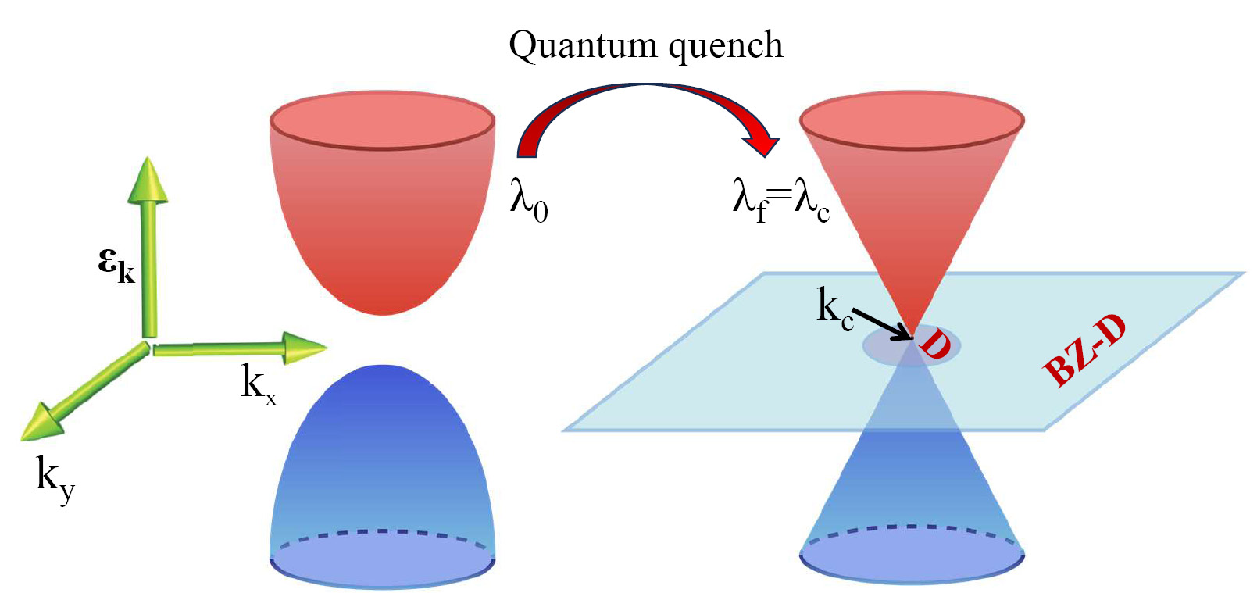
\includegraphics[width=0.7\textwidth]{figures/QV_BZ_D.pdf}
				\centering
				\bicaption{二维系统量子淬火动力学的示意图}{Illustration of the quantum quench dynamics in a 2D case} \label{Fig:BZ_D}
			\end{figure} 
		
		%\bicaption{二维系统量子淬火动力学的示意图。
			%阴影部分(区域$D$)表示了第一布里渊区中能隙闭合点$\mathbf{k}_c$附近的邻域。}{Illustration of the quantum quench dynamics in a 2D case.
			%The shadowed regime (denoted by $D$) indicates a small vicinity around the gap close point $\mathbf{k}_c$ in the 1st BZ.} \label{Fig:BZ_D}		
		
			{\bf 第一步:}
			哈密顿矢量${\vec{h}}_{\mathbf{k}}$的解析性允许我们将积分区间从整个第一布里渊区缩小到孤立能隙闭合点的邻域内。
			一般来说,对于任意的维度,公式\eqref{Eq:v}和Eq.~\eqref{eq:Cd}的积分范围可以被缩小到第一布里渊区的一个开子集$S$,只要$S$包含了第一布里渊区的所有能隙闭合点,不管这些能隙闭合点是否是孤立的。
			简单起见,考虑第一布里渊区内只有一个能隙闭合点,我们需要证明:
			\begin{equation}\label{eq:BZ-D}
				\frac{d}{d\lambda_f} \int_{BZ-D} r_\mathbf{k}(\lambda_f) d\mathbf{k} \bigg|_{\lambda_f=\lambda_c^-} - \frac{d}{d\lambda_f} \int_{BZ-D} r_\mathbf{k}(\lambda_f) d\mathbf{k} \bigg|_{\lambda_f=\lambda_c^+}
			\end{equation}
			这一表达式为零。
			其中$D$是$\mathbf{k}_c$附近任意小的邻域。
			对于更高的维度,讨论的思路也是类似的。
			对于$D$关于第一布里渊区的补集$BZ-D$,$r_\mathbf{k}^2$是关于$\mathbf{k} \in BZ-D$和$\lambda \in (\lambda_c-\delta \lambda, \lambda_c+\delta \lambda)$双重解析的函数,所以$r_\mathbf{k}=\sqrt{R_\mathbf{k}}$和${\partial r_\mathbf{k}(\lambda_f)}/{\partial \lambda_f}$是有界的,于是关于$k$的积分和关于$\lambda_f$的导数可以交换:
			\begin{equation}
				\int_{BZ-D} \left(\frac{\partial r_\mathbf{k}(\lambda_f)}{\partial\lambda_f}  \bigg|_{\lambda_f = \lambda_c^-} - \frac{\partial r_\mathbf{k}(\lambda_f)}{\partial\lambda_f} \bigg|_{\lambda_f=\lambda_c^+}\right) d\mathbf{k}
			\end{equation}
			这部分贡献只能来自$R_\mathbf{k}(\lambda_c)$的零点,因为不解析性来自于对$R_\mathbf{k}(\lambda_c)$开根号。
			由于$R_\mathbf{k}(\lambda_c)$在$BZ-D$内是解析的且不恒为0,足以说明这些零点构成的是一个零测集,因此公式~\eqref{eq:BZ-D}的值为零。
			至此,我们得到了
			\begin{equation}
				\frac{d}{d\lambda_f} v(\lambda_f) \bigg|_{\lambda_f=\lambda_c^-} - \frac{d}{d\lambda_f} v(\lambda_f) \bigg|_{\lambda_f=\lambda_c^+}=\frac{d}{d\lambda_f} \tilde{v}(\lambda_f) \bigg|_{\lambda_f=\lambda_c^-} - \frac{d}{d\lambda_f} \tilde{v}(\lambda_f) \bigg|_{\lambda_f=\lambda_c^+},
			\end{equation}
			其中
			\begin{equation}\label{Eq:v_reduce}
				\tilde{v}(\lambda_f) \equiv \int_{D}{r_\mathbf{k}(\lambda_f) d\mathbf{k}},
			\end{equation}
			基于公式~\eqref{Eq:v_reduce},我们就可以对$r_\mathbf{k}$在能隙闭合点$k_c$附近进行泰勒展开,以简化后续计算。
			
			{\bf 第二步:}
			能隙闭合点的简单结构假设可以显著简化计算的过程。
			不失一般性地,我们可以通过$\mathbf{k}$和$\lambda_f$的变量代换使得$k_c=0$,$\lambda_c=0$。
			对于一维系统,我们对能隙闭合点的简单结构定义为:
			$\exists \delta \lambda, \forall \lambda \in (- \delta \lambda, \delta \lambda)$,使得$\epsilon_k^2$的泰勒展开满足:
			\begin{equation}
				\epsilon_k^2 = f(\lambda) k^{2n} + l(\lambda) + o(k^{2n}),
			\end{equation}
			其中$n$是$k$的最低次数,且
			\begin{equation}
				\begin{aligned}
					& \lim_{\lambda \rightarrow 0^-}{f(\lambda)} = \lim_{\lambda \rightarrow 0^+}{f(\lambda)} \equiv f(\lambda=0)\neq0,\\
					& \lim_{\lambda \rightarrow 0^-}{l(\lambda)} = \lim_{\lambda \rightarrow 0^+}{l(\lambda)} \equiv l(\lambda=0)=0.
				\end{aligned}
			\end{equation}
			这一条件意味着在泰勒展开的收敛域内,只要$k \neq k_c$或$\lambda \neq \lambda_c$,就有$\epsilon_k \neq 0$,而$\epsilon_k = 0$当且仅当$k=k_c$且$\lambda=\lambda_c$。
			这也排除了多个局域的极值点随着$\lambda$逼近$\lambda_c$收敛到同一个能隙闭合点的可能性。
			能隙闭合点简单结构的物理含义是明确的:$\lambda\rightarrow\lambda_c$时低能有效理论的形式是收敛的,这一点对于大量符合场论描述的格点模型都是成立的。
			哈密顿矢量${\vec{h}}_{\mathbf{k}}$的泰勒展开可以被一般地表示为
			\begin{equation}
				\vec{h}_k = [k^{n_X}(a_X \lambda + b_X) + o(k^{n_X}),
				k^{n_Y}(a_Y \lambda + b_Y) + o(k^{n_Y}),
				k^{n_Z}(a_Z \lambda + b_Z) + o(k^{n_Z})].
			\end{equation}
			既然当$\lambda=0$时,只要$k \neq 0$就有$\vec{h}_k \neq \mathbf{0}$,那么$\{n_X,n_Y,n_Z\}$这三个数中至少存在一个非零的数。
			于是下面我们进行分类讨论。
			\begin{enumerate}
				\item $\{n_X,n_Y,n_Z\}$中只有一个数为0。
				不失一般性地,通过SU$(2)$的基底变换,我们总能选取$n_Z=0$因此由于能隙在$\lambda_c = 0$处闭合所以$b_Z$必须为0。
				\begin{enumerate}
					\item 如果$n_X > n_Y$,那么对应的色散关系就是$\epsilon_k^2 \sim k^{2n_X}(a_X \lambda + b_X)^2 + k^{2n_Y}(a_Y \lambda + b_Y)^2 + \lambda^2$。(对于$n_X < n_Y$的讨论也是类似的。)
					\begin{enumerate}
						\item 如果$\epsilon_k^2$的主导项是拥有非零系数$(a_X\lambda+b_X)$的$k^{2n_X}$,那么必须要求$a_Y=b_Y=0$。
						不仅如此,$\sigma^Z$前面的高阶项必须被限制在$o(k^{2n_X})$。
						从简单结构假设出发还要求$b_X\neq0$。
						由于我们关心$\delta\lambda\ll1$的情况,于是我们可以忽略$a_X \lambda$。
						最后,哈密顿矢量可以被简化为$\vec{h}_k = [b_X k^{n_X} + o(k^{n_X}),0,\lambda + o(k^{2n_X})]$,其中$\lambda$的系数已经被归一化。
						\item 如果$\epsilon_k$的主导项是$k^{2n_Y}$,那么要求$b_Y \neq 0$,且出于和前一种情形同样的理由,$a_Y \lambda$可以被忽略。
						因此,哈密顿矢量可以被简化为$\vec{h}_k = [o(k^{n_Y}), b_Y k^{n_Y} + o(k^{n_Y}),\lambda + o(k^{2n_Y})]$。
					\end{enumerate}
					\item 如果$n_X = n_Y \ \dot= \ n$,那么通过一个SU$(2)$的基地变换,哈密顿矢量可以被简化为$\vec{h}_k = [\sqrt{b_X^2+c_Y^2} k^{n} + o(k^{n}), o(k^{n}),\lambda+ o(k^{2n})]$。
				\end{enumerate}
				\item $\{n_X,n_Y,n_Z\}$之中有两个数为0。
				不失一般性地,由于$\lambda_c = 0$我们可以假设$n_Y=n_Z=0$并且将$b_Y,b_Z$也设置为0。
				那么通过一个与$k$无关的基底变换,就可以得到哈密顿矢量的简化形式为$\vec{h}_k = [b_X k^{n_X} + o(k^{n_X}),0,\lambda + o(k^{2n_X})]$。
			\end{enumerate}
			总结以上的所有情况,我们可以得到$\vec{h}_k$的简化形式为:
			\begin{equation} \label{h_k_reduce_1D}
				\vec{h}_k = [J k^{n} + o(k^{n}), o(k^{n}), \lambda + o(k^{2n})].
			\end{equation}
		
			对于二维的系统,能隙闭合点的简单结构被定义为:
			当$\lambda \rightarrow \lambda_c$时,$\epsilon_\mathbf{k}^2$的泰勒展开形式可以被表示为
			\begin{equation}
				\epsilon_\mathbf{k}^2 = f_x(\lambda) k_x^\alpha + f_y(\lambda) k_y^\beta + g(\lambda) + o(k_x^\alpha) + o(k_y^\beta),
			\end{equation}
			其中$\alpha,\beta$是$k_x,k_y$的最低次数,且
			\begin{equation}
				\begin{aligned}
					& \lim_{\lambda \rightarrow \lambda_c^-}{f_{x(y)}(\lambda)} = \lim_{\lambda \rightarrow \lambda_c^+}{f_{x(y)}(\lambda)} \equiv f_{x(y)}(\lambda_c)\neq0,\\
					& \lim_{\lambda \rightarrow \lambda_c^-}{g(\lambda)} = \lim_{\lambda \rightarrow \lambda_c^+}{g(\lambda)} \equiv g(\lambda_c)=0.
				\end{aligned}
			\end{equation}
			和一维的情形类似,既然$\vec{h}_\mathbf{k}$中$k_x,k_y$的交叉项会对$\epsilon_\mathbf{k}$的收敛行为产生贡献,哈密顿矢量的泰勒展开通常可以被表示为
			\begin{equation}
				\vec{h}_\mathbf{k} = k_x^{\vec{\alpha}}(\vec{a} \lambda + \vec{b}) + k_y^{\vec{\beta}}(\vec{c} \lambda + \vec{d}) + o(k_x^{\vec{\alpha}} ,k_y^{\vec{\beta}}),
			\end{equation}
			类似地,$\{(\alpha_X,\beta_X),(\alpha_Y,\beta_Y),(\alpha_Z,\beta_Z)\}$之中至少有一个非零矢量。
			接下来我们进行分类讨论:
			\begin{enumerate}
				\item $\{(\alpha_X,\beta_X),(\alpha_Y,\beta_Y),(\alpha_Z,\beta_Z)\}$之中只有一个零矢量。
				不失一般性地,假设$\alpha_Z=0,\beta_Z=0$,且由于$\lambda_c = 0$我们可以将$b_Z,d_Z$设置为0。
				\begin{enumerate}
					\item 按照一维情况下的分析,如果$\alpha_X \neq \alpha_Y$,
					$k_x^{\alpha_X}(a_X \lambda + b_X)$和$k_x^{\alpha_Y}(a_Y \lambda + b_Y)$之中只有其中一项能被留下。
					然而,如果在这种情况下$k_x$和$k_y$出现在相同的泡利矩阵之前,那么$k_x,k_y$的交叉项就会进入$\epsilon_\mathbf{k}$的表达式,这和简单结构假设是矛盾的。
					于是哈密顿矢量的一种等价表示是$\vec{h}_\mathbf{k} = [k_x^{\alpha}(a_X \lambda + b_X) + o(k_x^{\alpha}, k_y^{\beta}),  k_y^{\beta}(c_Y \lambda + d_Y) + o(k_x^{\alpha}, k_y^{\beta}), \lambda + o(k_x^{2\alpha}, k_y^{2\beta})]$。
					对于$\beta_X \neq \beta_Y$的分析也是类似的。
					\item 如果$\alpha_X = \alpha_Y \ \dot= \ \alpha, \beta_X = \beta_Y
					\ \dot= \ \beta$,$\epsilon_\mathbf{k}$中的交叉项就会是$2(b_X d_X + b_Y d_Y)k_x^\alpha    k_y^{\beta}$,这要求$b_X d_X + b_Y d_Y = 0$。
					得益于SU(2)对称性,不同泡利矩阵前面的$k_x$和$k_y$可以通过一个旋转变换被解耦。
				\end{enumerate}
				\item $\{(\alpha_X,\beta_X),(\alpha_Y,\beta_Y),(\alpha_Z,\beta_Z)\}$之中只有一个非零矢量。
				这种情况下,$k_x,k_y$的交叉项总会出现在$\epsilon_\mathbf{k}^2$,应当被排除。
			\end{enumerate}
			总结起来,二维情况下的哈密顿矢量可以的简化形式是
			\begin{equation} \label{h_k_reduce_2D}
				\vec{h}_k = [J_{k_x} k_x^{\alpha} + o(k_x^{\alpha} ,k_y^{\beta}), J_{k_y} k_y^{\beta} + o(k_x^{\alpha} ,k_y^{\beta}), \lambda + o(k_x^{2\alpha} ,k_y^{2\beta})].
			\end{equation}
		
			{\bf 第三步:}
			基于公式~\eqref{h_k_reduce_1D}和\eqref{h_k_reduce_2D}中哈密顿矢量$\vec{h}_k$的简化形式,忽略高阶项(由于我们关心$k_c$附近的小邻域)之后,我们就可以推导出量子态体积增长率的解析形式以及普适常数$C_d$。
			
			%我们先给出量子态体积一般的量子淬火动力学。
			从哈密顿矢量最初的形式$\hat{\mathcal{H}}_k(\lambda)=\vec{h}_\mathbf{k}\cdot \vec{\sigma}$出发,我们可以得到基态的色散关系为$\epsilon_k^{\pm}=\pm|\vec{h}_\mathbf{k}|$。
			方便起见,我们记$\epsilon_\mathbf{k}=|\vec{h}_\mathbf{k}|$。
			假设初态是$\hat{\mathcal{H}}_\mathbf{k}(\lambda_0)$的基态,那么对应的波函数为
			\begin{equation}\label{phi0}
				|u_\mathbf{k}^0 \rangle=
				\left[\sqrt{\frac{{{\epsilon_0}_\mathbf{k}-{h_0}_\mathbf{k}^z}}{2{\epsilon_0}_\mathbf{k}}},
				\frac{{h_0}_\mathbf{k}^x+ i {h_0}_\mathbf{k}^y}{\sqrt{2{\epsilon_0}_\mathbf{k}({\epsilon_0}_\mathbf{k}-{h_0}_\mathbf{k}^z)}}\right],
			\end{equation}
			其中$i$是虚数单位。
			根据前文叙述的两条假设,我们可以推导出对于二维系统:
			\begin{equation} \label{Eq:rk_2D}
				r_\mathbf{k} = \frac2\pi \sqrt{R_\mathbf{k}} =\frac{\left|({\vec{h}}_{0\mathbf{k}} \times {\vec{h}}_{f\mathbf{k}}) \cdot (\frac{\partial {\vec{h}}_{f\mathbf{k}}}{\partial x} \frac{\partial \epsilon_\mathbf{k}}{\partial y} - \frac{\partial {\vec{h}}_{f\mathbf{k}}}{\partial y} \frac{\partial \epsilon_\mathbf{k}}{\partial x})\right|}{\pi|{\vec{h}}_{0\mathbf{k}}| \cdot |{\vec{h}}_{f\mathbf{k}}|^2},
			\end{equation}
			其中$x, y$指$k_x, k_y$。
			将第二步得到的哈密顿矢量简化形式代入,可以得到
			\begin{equation}
				\tilde{v}_{2D} = \int_{D}{\frac{\alpha \beta |\lambda_f-\lambda_0||J_{k_x}J_{k_y}k_x^{\alpha-1} k_y^{\beta-1}|(J_{k_x}^2k_x^{2\alpha}+J_{k_y}^2k_y^{2\beta})}{\pi(\lambda_f^2+J_{k_x}^2k_x^{2\alpha}+J_{k_y}^2k_y^{2\beta})^{\frac32}(\lambda_0^2+J_{k_x}^2k_x^{2\alpha}+J_{k_y}^2k_y^{2\beta})^{\frac12}} d\mathbf{k}}.
			\end{equation}
			$(\lambda_0^2+k_x^{2\alpha}+k_y^{2\beta})^{\frac12}$这一项可以用其在$\mathbf{k}_c$处的值$|\lambda_0|$来代替。
			由于我们关心$\lambda_f$趋近于$\lambda_c$的行为,所以$|\frac{\lambda_f-\lambda_0}{\lambda_0}|$可以用1来代替。
			通过变量代换$k_x'=J_x k_x^\alpha,k_y'=J_y k_y^\beta$和一个极坐标变换$k_x'=q\cos{\theta},k_y'=q\sin{\theta}$,我们得到量子态体积的增长率为
			\begin{equation}
				\tilde{v}_{2D} = \int_{0}^{\Lambda}{\frac{2q^3}{(\lambda_f^2+q^2)^\frac32}}dq
				= \frac{4(\sqrt{\lambda_f^2+\Lambda^2}-|\lambda_f|)^2}{\sqrt{\lambda_f^2+\Lambda^2}},
			\end{equation}
			进一步计算就可以得到一维的普适常数$C_2=8$。			
			
			而对于一维系统,公式~\eqref{eq:Rk}退化为
			\begin{equation}
				\mathbb{B}(k) = f_k^0(t)+f_k^1(t) t+R_k t^2,
			\end{equation}
			其中
			\begin{equation} \label{Eq:rk_1D}
				r_k = \sqrt{R_k} = \frac{|{\vec{h}}_{0k}\times \vec{h}_{fk}||\dot{\epsilon}_k|}{|{\vec{h}}_{0k}|\cdot|\vec{h}_{fk}|},
			\end{equation}
			$\dot{\epsilon}_k$表示对$k$的导数。
			将第二步得到的哈密顿矢量简化形式代入,可以得到
			\begin{equation}
				\tilde{v}_{1D} = \int_{-\Lambda}^{\Lambda}{\frac{n |\lambda_f-\lambda_0||J k^{n-1}|J^2 k^{2n}}{(\lambda_f^2+J^2 k^{2n})^{\frac32}(\lambda_0^2+J^2 k^{2n})^{\frac12}} dk}.
			\end{equation}
			$(\lambda_0^2+J^2 k^{2n})^{\frac12}$这一项可以用其在$k_c$处的值$|\lambda_0|$来代替。
			由于我们关心$\lambda_f$趋近于$\lambda_c$的行为,所以$|\frac{\lambda_f-\lambda_0}{\lambda_0}|$可以用1来代替。
			通过一个变量代换$k_x'=J k_x^\alpha$,我们得到量子态体积的增长率为
			\begin{equation}
				\tilde{v}_{1D} = \int_{0}^{\Lambda^n}{\frac{2k_x'^2}{\lambda_f^2+k_x'^2}}dk_x'
				= 2\left(\Lambda^nJ-\lambda_f\arctan{\frac{\Lambda^nJ}{\lambda_f}}\right),
			\end{equation}
			进一步计算就可以得到一维的普适常数$C_1=2\pi$。
			至此我们就推导出了公式~\eqref{eq:cd}的结果。
			
		\subsection{数值结果}
			除了解析上的证明以外,我们还通过数值计算了一些具体的模型来验证我们的结论。
			我们考虑了一些一维和二维的被广泛研究过的模型。
			第一个一维的例子是一维的Kitaev链~\cite{Kitaev2001},它可以用公式~\eqref{eq:Ham}中的k空间哈密顿量来刻画。
			在这个模型中,$C_k = [c_k, c_{-k}^\dag]$表示的是南部表象下的无自旋费米子算符,哈密顿量可以写成~\cite{Kitaev2001}
			\begin{equation}
				\vec{h}(k) = [0, i\Delta\sin k, J\cos k + \lambda(t)],
			\end{equation}
			其中$J$和$\Delta$分别代表近邻格点跃迁强度和配对强度。
			简单起见,我们假设$\Delta = J$。
			$\lambda(t)$项代表化学势,是一个可以在时间维度上调节的参数。
			这个模型在临界点$\lambda_c = J$处展现出了基态拓扑量子相变,其中能隙在$k_c = \pi$处闭合。
			在临界点附近,能谱的色散关系可以近似为$\epsilon_k \sim J|k - k_c|$。
			我们研究了这个模型的量子淬火动力学,从控制参数$\lambda=\lambda_0$对应的哈密顿量的基态出发,将$\lambda$突然调整到$\lambda_f$,研究在系统在新哈密顿量下的演化行为。
			从相同的初态出发,在不同$\lambda_f$下对应的量子态体积$g_{1D}(t)$的演化如图~\ref{fig:QV_1D_kitaev}~(a)所示。
			$g_{1D}(t)$呈现出了线性增长。
			如图\ref{fig:QV_1D_kitaev}~(b)所示,增长率$v$是$\lambda_f$的函数,且在量子临界点$\lambda_f=J$处有一个弯折。
			这个弯折具体来看是$v(\lambda_f)$对$\lambda_f$的导数在$\lambda_f=\lambda_c$出现了不连续的行为,如图~\ref{fig:QV_1D_kitaev}~(b)的内页所示。
			更重要的是图~\ref{fig:QV_1D_kitaev}~(c)中所展示的,从不同的$\lambda_0$对应初态出发的动力学,在量子临界点处$g_{1D}(t)$对$\lambda_f$一阶导数的跳变都是$C_1=2\pi$。
			
			\begin{figure}[!htp]
				\centering
				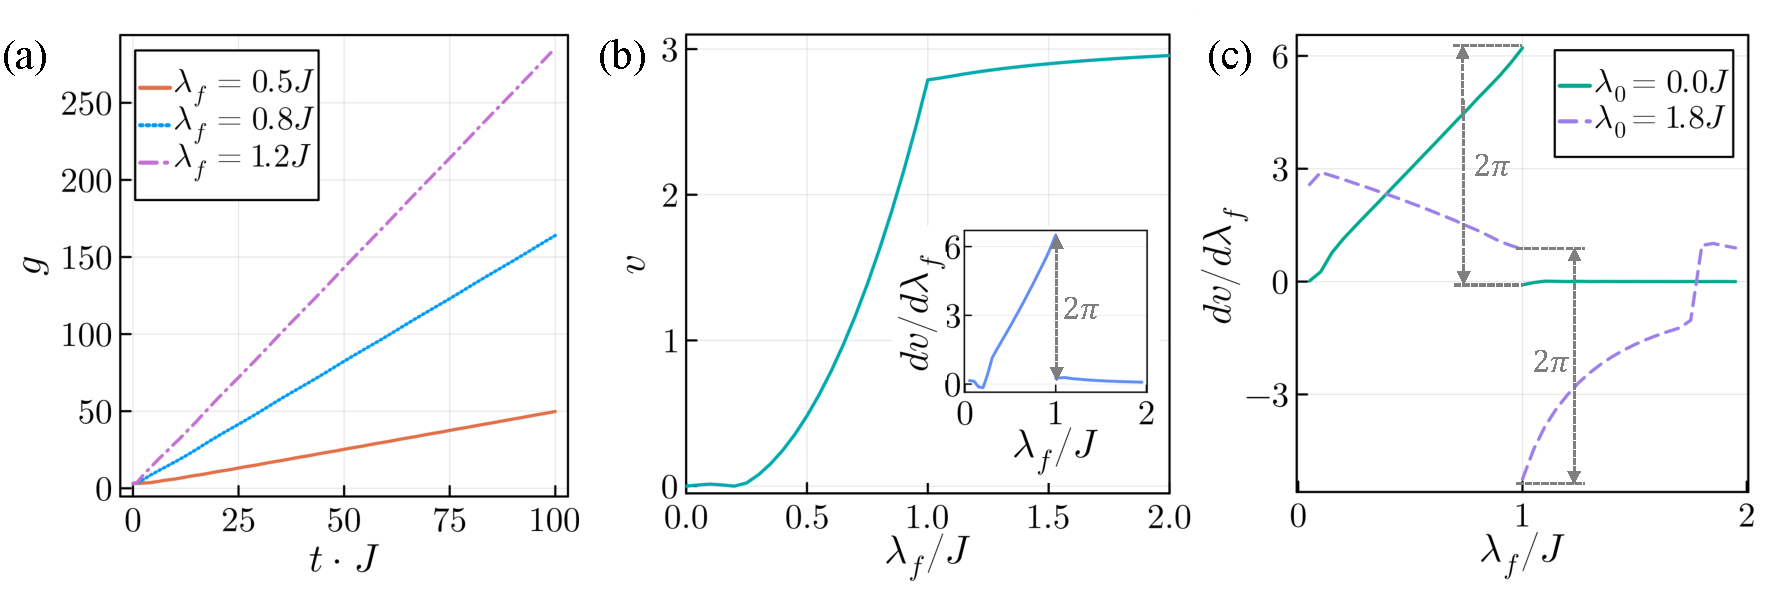
\includegraphics[width=1\textwidth]{figures/QV_1D_kitaev.pdf}
				\centering
				\bicaption{(a) 一维Kitaev模型从相同的初态$\lambda_0=0.2J$淬火到不同的$\lambda_f$对应的哈密顿量下量子态体积 $g(t)$随时间的演化。
					(b) 增长率$v$与不同$\lambda_f$之间的关系。内页是增长率$v$关于$\lambda_f$的导数,其在量子临界点处展现出了普适的跳变值$2\pi$。
					(c) 从不同$\lambda_0$对应的初态出发,$dv/d\lambda_f$随着$\lambda_f$的变化关系,且在 $\lambda_f=J$展现出了相同跳变值$2\pi$。}
					{(a) Quantum state volume $g(t)$ for the 1D Kitaev model in the quantum quench dynamics starting from the same initial states with $\lambda_0=0.2J$, but evolving under the Hamiltonian with different $\lambda_f$.
					(b) The growth velocity $v$ as a function of $\lambda_f$. The inset is its derivative with respect to $\lambda_f$ , which exhibits a discontinuity with an universal jump value $2\pi$.
					(c) $dv/d\lambda_f$ as a function of $\lambda_f$ starting from initial states with different $\lambda_0$, which share the same jump value of $2\pi$ at $\lambda_f=J$.}
				\label{fig:QV_1D_kitaev}
			\end{figure}
		
			第二个一维的例子是Su-Schrieffer-Heeger~(SSH)模型,它的哈密顿量是
			\begin{equation}
				H = \lambda\sum_{i=1}^{N}{c^\dagger_{i,A}c_{i,B}} + J\sum_{i=1}^{N}{c^\dagger_{i+1,A}c_{i,B}} + h.c.
			\end{equation}
			其中$i$是元胞的指标,每个元胞包含了A和B两种不同的格点。
			我们选择周期边界条件$c^\dagger_{N+1,A/B} = c^\dagger_{1,A/B}$之后,就可以通过傅里叶变换得到动量空间下的哈密顿矢量为$\vec{h}_k = (\lambda+J\cos{k},J\sin{k},0)$,其中第一布里渊区的范围是$k \in [0,2\pi)$。
			不失一般性地,我们考虑$\lambda > 0$且$J > 0$,于是哈密顿矢量被约化为$\vec{h}_k = (\lambda,Jk,0)$。
			当$\lambda_c=J$且$k_c=\pi$时,能隙闭合。
			我们从数值上检验了$C_1 = 2\pi$,如图~\ref{Fig:QV_1D_SSH}~(a)所示,并且这个结果对于不同的$\lambda_0$都是成立的,如图~\ref{Fig:QV_1D_SSH}~(b)所示。
			
			\begin{figure}[!htp]
				\centering
				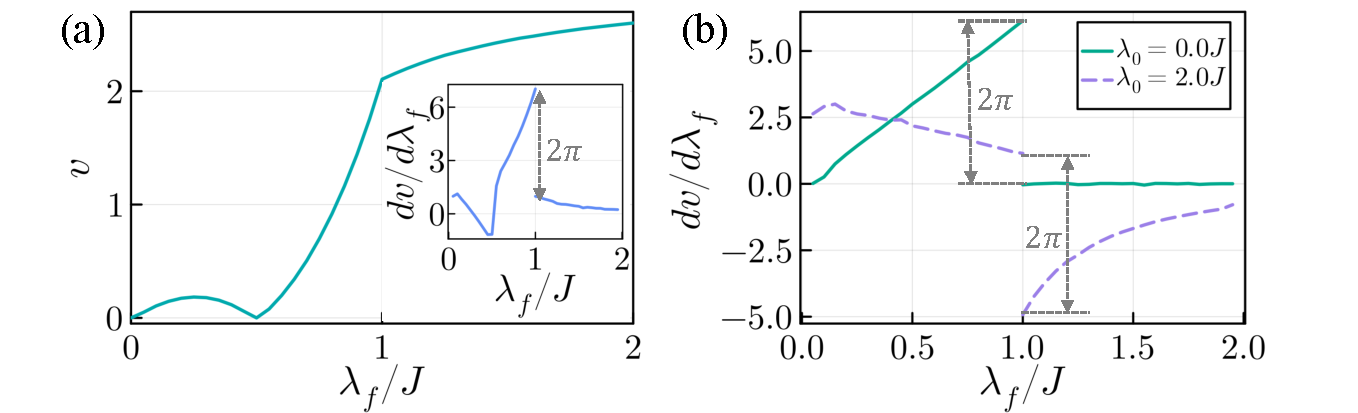
\includegraphics[width=1\textwidth]{figures/QV_1D_SSH.pdf}
				\centering
				\bicaption{(a) 当$\lambda_0 = 0.5J$时,线性增长的斜率随着$\lambda_f$的变化关系,并在$\lambda_f = 1.0J$处呈现出弯折。
					(b) 不同$\lambda_0$的跳变示意图,跳变值均为$2\pi$。}
				{(a) When $\lambda_0 = 0.5J$, the slope of linear growth with respect to $\lambda_f$, which exhibits a kink at $\lambda_f = 1.0J$.
					Inset: The derivative of the main set over $\lambda_f$, showing that the jump of slope at $\lambda_f = 1.0J$ equals $2\pi$.
					(b) The illustration of slope jumps at different $\lambda_0$, which all are equivalent to $2\pi$.}
				\label{Fig:QV_1D_SSH}
			\end{figure}
			
			最后一个一维的例子是带有周期交错化学势的费米子格点模型,它的哈密顿量是
			\begin{equation}
				H = -J\sum_{i=1}^{N}{c^\dagger_{i}c_{i+1}} + h.c. + (-1)^i\lambda\sum_{i=1}^{N}{c^\dagger_{i}c_{i}}
			\end{equation}
			考虑周期边界条件$c^\dagger_{N+1} = c^\dagger_{1}$之后,可以通过傅里叶变换得到动量空间的哈密顿矢量为$\vec{h}_k = (\lambda,0,2J\cos{k})$,其中第一布里渊区的范围是$k \in [0,\pi]$。
			不失一般性地,我们考虑$J > 0$,于是哈密顿矢量可以被约化为$\vec{h}_k = (\lambda,0,-2Jk)$。
			当$\lambda_c=0$且$k_c=\pi/2$,系统的能隙闭合。
			我们从数值上验证了$C_1 = 2\pi$,如图~\ref{Fig:QV_1D_AB}~(a)所示,结论对于不同的$\lambda_0$都是成立的,如图~\ref{Fig:QV_1D_AB}~(b)所示。
			
			\begin{figure}[!htp]
				\centering
				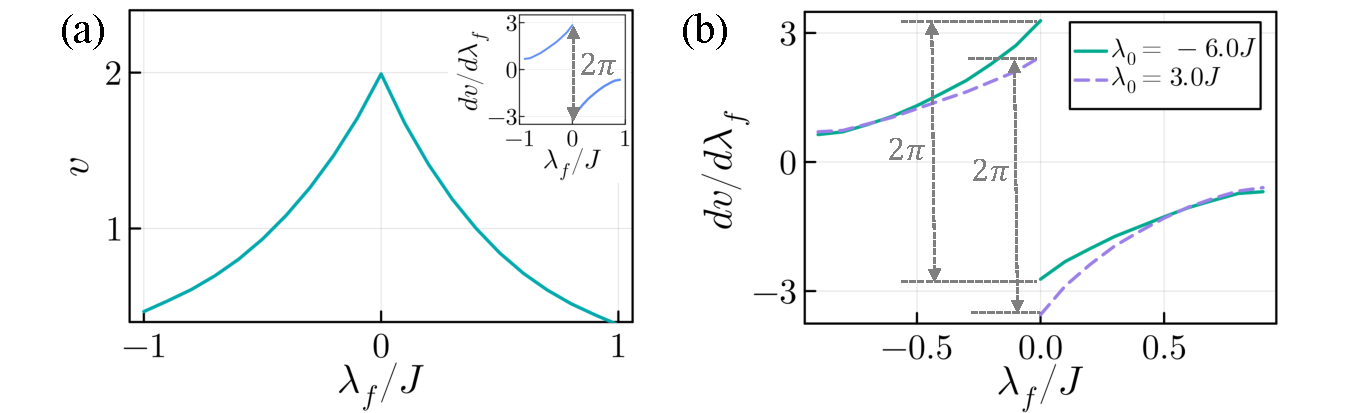
\includegraphics[width=1\textwidth]{figures/QV_1D_AB.pdf}
				\centering
				\bicaption{(a) 当$\lambda_0 = 10J$时,线性增长的斜率随着$\lambda_f$的变化关系,并在$\lambda_f = 0.0J$处呈现出弯折。
					(b) 不同$\lambda_0$的跳变示意图,跳变值均为$2\pi$。}
				{(a) When $\lambda_0 = 10.0J$, the slope of linear growth with respect to $\lambda_f$, which exhibits a kink at $\lambda_f = 0.0J$.
					Inset: The derivative of the main set over $\lambda_f$, showing that the jump of slope at $\lambda_f = 0.0J$ equals $2\pi$.
					(b) The illustration of slope jumps at different $\lambda_0$, which all are equivalent to $2\pi$.}
				\label{Fig:QV_1D_AB}
			\end{figure}
		
			对于二维的情形,我们也对两个不同的模型进行了计算。
			第一个模型是Qi-Wu-Zhang (QWZ)模型~\cite{Qi2006},它的哈密顿量是
			\begin{equation}
				\vec{h}_{QWZ}(\mathbf{k}) = [J\sin k_x, J\sin k_y, J(\cos k_x + \cos k_y) + \lambda(t)],\label{eq:QWZ}
			\end{equation}
			其中第一布里渊区的范围是$(k_x, k_y) \in (-\pi, \pi]$。
			这个模型分别在$\lambda = 0, \pm2J$处展现出了量子相变。
			对于$\lambda = 0$的情况,第一布里渊区内有两个能隙闭合点,即$\mathcal{N}=2$:$\mathbf{k}_c^1=(0,\pi)$和$\mathbf{k}_c^2=(\pi,0)$;
			而对于$\lambda = 2J(-2J)$的情况,第一布里渊区内就只有一个能隙闭合点,即$\mathcal{N}=1$,位于$\mathbf{k}_c=(0,0)$ ($\mathbf{k}_c=(\pi,\pi)$)。
			我们从公式\eqref{eq:QWZ}所描述的哈密顿量在控制参数$\lambda = \lambda_0$下的基态出发,然后突然将控制参数调节到$\lambda_f$,再让系统在这个新哈密顿量下演化,研究量子态体积$g(t)$的淬火动力学。
			$g(t)$依旧展现出了随时间的线性增长,如图~\ref{Fig:QV_2D_QWZ}~(a)所示。
			然后我们得到增长率$v(\lambda_f)$关于$\lambda_f$的导数。
			图~\ref{Fig:QV_2D_QWZ}~(b)和(c)说明了在$\lambda_f=-2J$和$\lambda_f=0$处分别出现了普适的跳变值,分别对应$\mathcal{N}=1$和$\mathcal{N}=2$的情形,与公式~\eqref{eq:Cd}中给出的结论$C_2 = 8$是一致的。
			
			\begin{figure}[!htp]
				\centering
				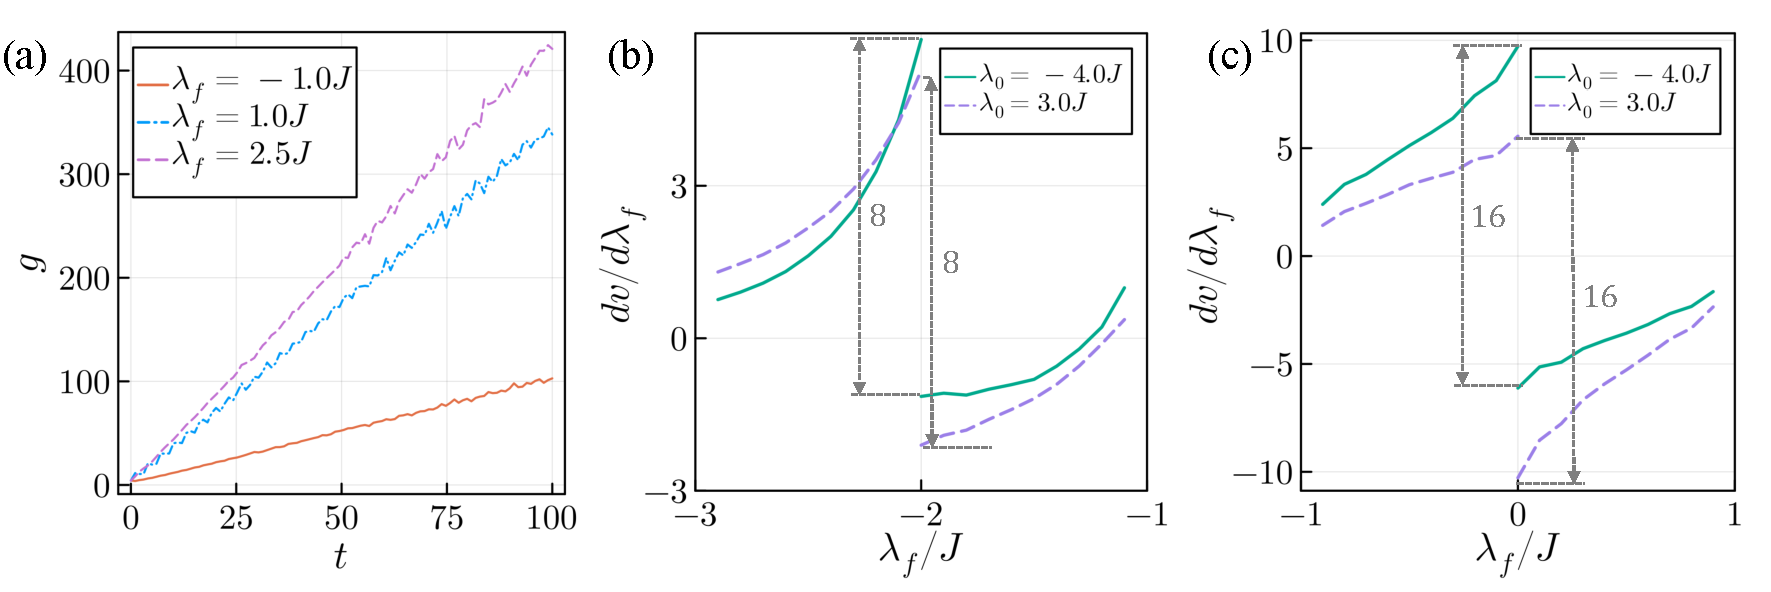
\includegraphics[width=1\textwidth]{figures/QV_2D_QWZ.pdf}
				\centering
				\bicaption{(a) 二维Qi-Wu-Zhang模型从相同的初态$\lambda_0=-0.5J$出发,在不同的哈密顿量$\lambda_f$下量子态体积的淬火动力学
					(b)和(c) $dv/d\lambda_f$随着$\lambda_f$在不同量子相变点(b) $\lambda_f=-2J$和(c) $\lambda_f=0$处的变化。
					$\lambda_f=-2J$ ($\lambda_f=0$)时,第一布里渊区内量子临界点的个数分别为$\mathcal{N}=1$ ($\mathcal{N}=2$)。}
				{(a) Quantum volume $g(t)$ for the 2D Qi-Wu-Zhang model in the quantum quench dynamics starting from the same initial states with $\lambda_0=-0.5J$, but evolving under the Hamiltonian with different $\lambda_f$.
					(b) and (c) $dv/d\lambda_f$ as a function of $\lambda_f$ around the different quantum critical points at (b) $\lambda_f=-2J$ and (c) $\lambda_f=0$.  The number of the gap closing points in the 1st BZ is $\mathcal{N}=1$ ($\mathcal{N}=2$) for the critical point at $\lambda_f=-2J$ ($\lambda_f=0$).}
				\label{Fig:QV_2D_QWZ}
			\end{figure}
		
	\section{结论与展望}
		总之,我们展示了量子临界性可以掌控远离基态的非平衡动力学,并诱导出普适的动力学行为。
		尽管量子体积依赖于无相互作用的能带结构,但其普适的速度跳跃完全由能隙闭合点附近的k渐近行为局部决定。
		因此,我们预期这种体积概念可以推广到存在相互作用的体系\cite{Souza2000},只要这些体系在临界点附近允许具有涌现平移对称性的有效场论描述,例如狄拉克物理和其他共形场论\cite{Francesco:2012aa,Wehling:2014aa}。
		而这正是在低维系统中普遍存在的特征\cite{Gogolin:2004aa}。
	
	
	
% !TEX root = ../main.tex

\chapter{全文总结}

这里是全文总结内容。


%TC:ignore

% 参考文献
\printbibliography[heading=bibintoc]

% 附录
\appendix

% 附录中图表不加入索引
% \captionsetup{list=no}

% 附录内容
% !TEX root = ../main.tex

\chapter{简单能带结构假设下二维量子态体积增长率的推导过程}

	这里我们给出简单能带结构假设下二维量子态体积增长率的推导过程。
	我们从公式\eqref{h_k_reduce_2D}给出的哈密顿矢量出发,简单起见,我们将$J_{k_x},J_{k_y}$设置为1,并忽略所有高阶项。
	我们还可以通过坐标变换,将$k_x,k_y$的次数$\alpha,\beta$变换成1。
	于是我们得到简化后的哈密顿矢量为
	\begin{equation} \label{h_k_rereduce_2D}
		\vec{h}_k = [k_x, k_y, \lambda]
	\end{equation}

	下面我们从这个哈密顿矢量出发进行量子态体积增长率的推导。
	通过对角化可以得到,淬火前系统位于$\lambda_0$所控制的初态
	\begin{equation}
		|\phi_k(0) \rangle =
		\left(
			\begin{array}{l}
				-\sqrt{\frac{\epsilon_{0k}^2-\lambda_0\epsilon_{0k}}{2\epsilon_{0k}}} \\ [10pt]
				\frac{x_k + iy_k}{2(\epsilon_{0k}^2-\lambda_0\epsilon_{0k})}
			\end{array}
		\right)
	\end{equation}
	上,其中$\epsilon_{0k} = \sqrt{x_k^2+y_k^2+\lambda_0^2}$是淬火前哈密顿量的色散关系。
%% % !TEX root = ../main.tex

\chapter{Maxwell Equations}

选择二维情况,有如下的偏振矢量:
\begin{subequations}
  \begin{align}
    {\bf E} &= E_z(r, \theta) \hat{\bf z}, \\
    {\bf H} &= H_r(r, \theta) \hat{\bf r} + H_\theta(r, \theta) \hat{\bm\theta}.
  \end{align}
\end{subequations}
对上式求旋度:
\begin{subequations}
  \begin{align}
    \nabla \times {\bf E} &= \frac{1}{r} \frac{\partial E_z}{\partial\theta}
      \hat{\bf r} - \frac{\partial E_z}{\partial r} \hat{\bm\theta}, \\
    \nabla \times {\bf H} &= \left[\frac{1}{r} \frac{\partial}{\partial r}
      (r H_\theta) - \frac{1}{r} \frac{\partial H_r}{\partial\theta} \right]
      \hat{\bf z}.
  \end{align}
\end{subequations}
因为在柱坐标系下,$\overline{\overline\mu}$ 是对角的,所以 Maxwell 方程组中电场
$\bf E$ 的旋度:
\begin{subequations}
  \begin{align}
    & \nabla \times {\bf E} = \ii \omega {\bf B}, \\
    & \frac{1}{r} \frac{\partial E_z}{\partial\theta} \hat{\bf r} -
      \frac{\partial E_z}{\partial r}\hat{\bm\theta} = \ii \omega \mu_r H_r
      \hat{\bf r} + \ii \omega \mu_\theta H_\theta \hat{\bm\theta}.
  \end{align}
\end{subequations}
所以 $\bf H$ 的各个分量可以写为:
\begin{subequations}
  \begin{align}
    H_r &= \frac{1}{\ii \omega \mu_r} \frac{1}{r}
      \frac{\partial E_z}{\partial\theta}, \\
    H_\theta &= -\frac{1}{\ii \omega \mu_\theta}
      \frac{\partial E_z}{\partial r}.
  \end{align}
\end{subequations}
同样地,在柱坐标系下,$\overline{\overline\epsilon}$ 是对角的,所以 Maxwell 方程
组中磁场 $\bf H$ 的旋度:
\begin{subequations}
  \begin{align}
    & \nabla \times {\bf H} = -\ii \omega {\bf D}, \\
    & \left[\frac{1}{r} \frac{\partial}{\partial r}(r H_\theta) - \frac{1}{r}
      \frac{\partial H_r}{\partial\theta} \right] \hat{\bf z} = -\ii \omega
      {\overline{\overline\epsilon}} {\bf E} = -\ii \omega \epsilon_z E_z
      \hat{\bf z}, \\
    & \frac{1}{r} \frac{\partial}{\partial r}(r H_\theta) - \frac{1}{r}
      \frac{\partial H_r}{\partial\theta} = -\ii \omega \epsilon_z E_z.
  \end{align}
\end{subequations}
由此我们可以得到关于 $E_z$ 的波函数方程:
\begin{equation}
  \frac{1}{\mu_\theta \epsilon_z} \frac{1}{r} \frac{\partial}{\partial r}
  \left(r \frac{\partial E_z}{\partial r} \right) + \frac{1}{\mu_r \epsilon_z}
  \frac{1}{r^2} \frac{\partial^2E_z}{\partial\theta^2} +\omega^2 E_z = 0.
\end{equation}

%% % !TEX root = ../main.tex

\chapter{绘制流程图}

图~\ref{fig:flow_chart} 是一张流程图示意。使用 \pkg{tikz} 环境,搭配四种预定义节
点(\verb|startstop|、\verb|process|、\verb|decision| 和 \verb|io|),可以容易地
绘制出流程图。

\begin{figure}[!htp]
  \centering
  \input{figures/flow_chart.tex}
  \bicaption{绘制流程图效果}{Flow chart}
  \label{fig:flow_chart}
\end{figure}


% 结尾部分
\backmatter

% 用于盲审的论文需隐去致谢、发表论文、科研成果、简历

% 致谢
% !TEX root = ../main.tex

\begin{acknowledgements}
  感谢那位最先制作出博士学位论文 \LaTeX{} 模板的物理系同学!

  感谢 William Wang 同学对模板移植做出的贡献!

  感谢 \href{https://github.com/weijianwen}{@weijianwen} 学长开创性的工作!

  感谢 \href{https://github.com/sjtug}{@sjtug} 对 0.10 及之后版本的开发和维护工作!

  感谢所有为模板贡献过代码的\href{https://github.com/sjtug/SJTUThesis/graphs/contributors}{同学们}, 以及所有测试和使用模板的各位同学!

  感谢 \LaTeX 和 \href{https://github.com/sjtug/SJTUThesis}{SJTUThesis},帮我节省了不少时间。
\end{acknowledgements}


% 发表论文及科研成果
% 盲审论文中,发表论文及科研成果等仅以第几作者注明即可,不要出现作者或他人姓名
% !TEX root = ../main.tex

\begin{achievements}

	\subsection*{学术论文}

		\begin{bibliolist}{00}
  			\item Chen H, Chan C~T. Acoustic cloaking in three dimensions using acoustic metamaterials[J]. Applied Physics Letters, 2007, 91:183518.
  			\item Chen H, Wu B~I, Zhang B, et al. Electromagnetic Wave Interactions with a Metamaterial Cloak[J]. Physical Review Letters, 2007, 99(6):63903.
		\end{bibliolist}

		\begin{bibliolist*}{00}
  			\item 第一作者. 中文核心期刊论文, 2007.
  			\item 第一作者. EI 国际会议论文, 2006.
		\end{bibliolist*}

\end{achievements}


%% 简历
%% % !TEX root = ../main.tex

\begin{resume}
  \subsection*{基本情况}
    某某,yyyy 年 mm 月生于 xxxx。

  \subsection*{教育背景}
  \begin{itemize}
    \item yyyy 年 mm 月至今,上海交通大学,博士研究生,xx 专业
    \item yyyy 年 mm 月至 yyyy 年 mm 月,上海交通大学,硕士研究生,xx 专业
    \item yyyy 年 mm 月至 yyyy 年 mm 月,上海交通大学,本科,xx 专业
  \end{itemize}

  \subsection*{研究兴趣}
    \LaTeX{} 排版

  \subsection*{联系方式}
  \begin{itemize}
    \item 地址: 上海市闵行区东川路 800 号,200240
    \item E-mail: \email{john_smith@sjtu.edu.cn}
  \end{itemize}
\end{resume}


% 学士学位论文要求在最后有一个大摘要,单独编页码
%% % !TEX root = ../main.tex

\begin{digest}
  An imperial edict issued in 1896 by Emperor Guangxu, established Nanyang
  Public School in Shanghai. The normal school, school of foreign studies,
  middle school and a high school were established. Sheng Xuanhuai, the person
  responsible for proposing the idea to the emperor, became the first president
  and is regarded as the founder of the university.

  During the 1930s, the university gained a reputation of nurturing top
  engineers. After the foundation of People's Republic, some faculties were
  transferred to other universities. A significant amount of its faculty were
  sent in 1956, by the national government, to Xi'an to help build up Xi'an Jiao
  Tong University in western China. Afterwards, the school was officially
  renamed Shanghai Jiao Tong University.

  Since the reform and opening up policy in China, SJTU has taken the lead in
  management reform of institutions for higher education, regaining its vigor
  and vitality with an unprecedented momentum of growth. SJTU includes five
  beautiful campuses, Xuhui, Minhang, Luwan Qibao, and Fahua, taking up an area
  of about \qty{3225833}{\square\metre}. A number of disciplines have been
  advancing towards the top echelon internationally, and a batch of burgeoning
  branches of learning have taken an important position domestically.

  Today SJTU has 31 schools (departments), 63 undergraduate programs, 250
  masters-degree programs, 203 Ph.D. programs, 28 post-doctorate programs, and
  11 state key laboratories and national engineering research centers.

  SJTU boasts a large number of famous scientists and professors, including 35
  academics of the Academy of Sciences and Academy of Engineering, 95 accredited
  professors and chair professors of the ``Cheung Kong Scholars Program'' and
  more than \num{2000} professors and associate professors.

  Its total enrollment of students amounts to \num{35929}, of which \num{1564}
  are international students. There are \num{16802} undergraduates, and
  \num{17563} masters and Ph.D. candidates. After more than a century of
  operation, Jiao Tong University has inherited the old tradition of ``high
  starting points, solid foundation, strict requirements and extensive
  practice.'' Students from SJTU have won top prizes in various competitions,
  including ACM International Collegiate Programming Contest, International
  Mathematical Contest in Modeling and Electronics Design Contests. Famous
  alumni include Jiang Zemin, Lu Dingyi, Ding Guangen, Wang Daohan, Qian Xuesen,
  Wu Wenjun, Zou Taofen, Mao Yisheng, Cai Er, Huang Yanpei, Shao Lizi, Wang An
  and many more. More than 200 of the academics of the Chinese Academy of
  Sciences and Chinese Academy of Engineering are alumni of Jiao Tong
  University.
\end{digest}


%TC:endignore

\end{document}
